\documentclass[10pt, singlespace]{harvard-thesis}
\usepackage{epsfig,amsmath,amssymb,multirow,color,xspace,fancyvrb,verbatim,url,listings,verbatim,alltt}

\special{papersize=8.5in,11in}
\setlength{\pdfpagewidth}{8.5in}
\setlength{\pdfpageheight}{11in}

\usepackage{enumerate}

\graphicspath{{./figures/}}

\newcommand{\tabitem}{~~\llap{\textbullet}~~}
\newcolumntype{L}[1]{>{\raggedright\let\newline\\\arraybackslash\hspace{0pt}}m{#1}}
\newcolumntype{C}[1]{>{\centering\let\newline\\\arraybackslash\hspace{0pt}}m{#1}}
\newcolumntype{R}[1]{>{\raggedleft\let\newline\\\arraybackslash\hspace{0pt}}m{#1}}

\newcounter{notecounter}
\newcommand{\mynote}[1]{\stepcounter{notecounter}\textcolor{red}{\small \bf [\arabic{notecounter}]}\marginpar{\tiny \sf \textcolor{red}{\bf [\arabic{notecounter}]}#1}}

\newcommand{\lyt}[1]{\mynote{LYT: #1}}

\begin{document}

% some details about the thesis
\title{Concurrency Algorithms in Transactional Data Structures}
\author{Lillian Tsai}
\advisor{Professor Eddie Kohler}

% about the degree
\degree{Bachelor of Arts}
\field{Computer Science}
\degreeyear{2017}
\degreemonth{May}

% about the university
\department{Department of Computer Science}
\university{Harvard University}
\universitycity{Cambridge}
\universitystate{Massachusetts}

\maketitle
\copyrightpage
\abstractpage

\tableofcontents
\listoffigures
\listoftables

\dedicationpage
\acknowledgments

%\onehalfspacing
\singlespacing

\chapter{Introduction}
\section{STM and STO}
Parallelism is increasingly critical for performance in computer software systems, but parallel programming remains enormously challenging to get right. Low-level mechanisms for coordinating threads, such as lock-based strategies, are fragile and error-prone. To address this problem, researchers have developed programming tools and methodologies for managing parallelism. Prominent among these is software transactional memory (STM), which allows programmers to write concurrent code using sequential programming paradigms. By using STM, programmers reason about concurrent operations on shared memory through transactions---atomic groups of operations---instead of single operations. 

Unfortunately, STM often results in high overhead and is rarely considered practical. To provide transactional guarantees, an STM system tracks the different memory words accessed within a transaction and ensures that these words are not touched by a separate, simultaneous transaction. Traditional word-based STM tracks all words of memory read or written in a transaction, incurring enormous overhead~\cite{cascaval}. To address this problem, a research team at Harvard has produced a novel type of STM, STO (Software Transactional Objects), that greatly improves upon the performance of traditional STM~\cite{sto}. The system's implementation works at a higher level than most previously developed systems: data structure operations, rather than individual memory words. For example, a word-STM tracks every word accessed in the path from the root during a binary search tree lookup, which leads to significant overhead from transactional bookkeeping and the introduction of unnecessary conflicts: the transaction will abort if there is a concurrent update to the path, even though the result of the lookup may be unaffected. STO allows datatypes to define datatype-specific abstract objects to track instead of memory words. Thus, during a binary search tree lookup, STO will track only the abstract object corresponding to the parent of the searched-for node, and use only this object to detect a conflict in which the node is modified, removed, or inserted. Compared to a word-STM, STO achieves both a reduced number of false conflicts and hundreds of times fewer objects to track.

\section{Motivation}
The focus of this work is to make STO as fast as the fastest concurrent programming patterns available, and when this is impossible, to characterize precisely why. Although STO outperforms traditional STM, STO’s performance still falls far below that of other concurrent programming paradigms such as Flat Combining~\cite{flatcombining}. STO’s library of transactional datatypes---datatypes exposing transactional operations---allows programmers to add transactional memory to their programs. Thus, STO programs are only as fast as STO's datatypes. A natural focus for our research is then transactional data structure algorithms: by defining the limits and potentials of these algorithms, we learn how to maximize the performance of the STO system.

\section{Overview}
While our research's scope includes all the different datatypes supported by STO, this thesis focuses on a few core data structures: queues and hashmaps. We first implemented the initial version of these STO datatypes and, more broadly, developed design techniques for transactional data structures. These techniques defined general patterns for designing transactional algorithms, such as how to handle reads and writes of the same object within the same transaction. These patterns, however, do not maximize scalability or performance.

To address our goal of performance maximization, we shifted our focus to analyze and compare the performance of existing STO data structures against implementations of highly-concurrent, non-transactional data structure algorithms from recent research. These concurrent data structure algorithms strive to maximize scalability and performance without the concern for transactional correctness: they ensure that single operations can execute concurrently in multiple threads but provide no guarantees that a thread can execute a sequence of operations (a transaction) without interruption from another thread (atomically).
Thus, the performance of the fastest concurrent datatypes available acts as an upper bound for the performance transactional STO data structures may reasonably hope to achieve. Our benchmarks highlight which concurrent, non-transactional data structures are the highest-performing, and which parts of the transactional data structure algorithms are bottlenecks and areas for improvement. 

We first hypothesize that combining concurrent, non-transactional programming patterns with our transactional design patterns will produce transactional datatypes that greatly outperform our previous implementations. To evaluate this hypothesis, we take the fastest concurrent datatype algorithms and implement them within the STO framework. We discover that the algorithmic changes necessary to move highly-parallel data structures into STO results in a significant decrease in their performance; at times, they even underperform our initial STO data structures that use naive algorithms for concurrency.
Furthermore, our experience combining highly-concurrent, non-transactional algorithms with transactional algorithms leads to the conclusion that reasoning about scalability in transactional datatypes is inherently different than reasoning about scalability in traditional concurrent datatypes. In particular, reasoning about invariants regarding datatype state is essential to handle transactions: a transactional algorithm must maintain state across operations within a transaction. We formalize this argument as a commutativity argument, drawing on previous work regarding commutativity in transactional objects~\cite{weihl}.

The stateful nature of transactions (and therefore reduced operation commutativity) leads us to revise our hypothesis. From our experimental results and experiences creating transactional data structures, it seems clear that the reasoning that allows a highly-concurrent data structure to achieve fast performance and scalability is intrinsically different from the reasoning required to create transactional, highly performant data structures. 
We claim that certain highly-concurrent algorithms for datatypes may be intrinsically non-transactional because the optimizations taken by these algorithms to achieve their high performances are incompatible with providing transactional guarantees. In other words, if the synchronization technique of a concurrent data structure interferes with the techniques required to support transactions, the data structure is unlikely to perform well in a transactional setting. Conversely, if the synchronization technique is mostly or completely independent of STO, meaning that transactional support can be added without modifying the synchronization algorithm itself, then we may still retain the benefits of the data structure's algorithmic optimizations in a transactional setting.

To evaluate our claim, we take highly-concurrent algorithms that underperformed when integrated with STO and investigate how these algorithms act when the transactional interface is modified. 
With an alternative interface, we achieve a better separation between the logic needed for transactional support and the logic of the concurrency algorithm: this allows us to adapt concurrent datatypes algorithms for transactional settings while retaining their high performance.
Redefining the transactional specification demonstrates the trade-offs between the guarantees STO datatypes can provide and their performance: for example, by preventing a thread from seeing its own writes (a violation of strong transactional guarantees), performance of the datatype more than doubles.
We also note that highly-concurrent algorithms whose core optimizations rely on reasoning independent from the reasoning used in our transactional techniques still provide performance benefits in the original transactional setting.

\subsection{Roadmap}
This work is divided into the following parts: 
\begin{itemize}
    \item Background information on transactions and transactional memory, and related work on transactional data structure algorithms and their scalability (Chapter~\ref{related_work})
    \item An evaluation of different transactional and concurrent algorithms for queue and hashmap data structures (Chapters~\ref{queue} and~\ref{hashmap})
    \item An explanation based on operation commutativity and invalid histories for why concurrent algorithms for queues fail to retain their performance benefits when moved into the STO transactional framework (Chapter~\ref{queue})
    \item A demonstration of how the performance loss of queue concurrent algorithms can be elided through changing the transactional specification (Chapter~\ref{commutativity})
    \item A demonstration of and explanation why highly-concurrent hashmap algorithms do, in fact, retain performance benefits in a transactional setting (Chapter~\ref{hashmap})
\end{itemize}


\chapter{Background and Related Work}
\label{related_work}

\section{Transactional Memory}
A transaction---a group of operations that together form one logical unit of work and have atomic effect---allows a programmer to reason more simply about concurrent access to shared state. The concept first developed in database theory, trickled into file systems, and then expanded to other domains with the development of hardware transactional memory (HTM) in 1986 and software transactional memory (STM) in 1995~\cite{harristm}. 
A transaction is commonly defined by the ACID properties: atomicity, consistency, isolation, and durability. Transactional memory (TM)~\cite{harristm, herlihytm} guarantees transactional properties in shared memory; this differs from transactions in a database which (traditionally) work with data on disk.
TM is therefore unconcerned with the durability property: memory does not persist on some permanent medium. However, TM must still adhere to the remaining three ACI properties:

\emph{Atomicity} ensures that, if a transaction commits, all changes made by the transaction are instantly visible to other actors performing transactions (for example, threads modifying shared memory or processes modifying a database). If a transaction aborts, none of the changes made by the transaction are visible to any other actor. Thus, either all or none of the operations of the transaction should appear to succeed.

\emph{Consistency} guarantees that a transaction begins and ends with the state of the database or data structure satisfying particular (data structure-specific) invariants: for example, an invariant could be that the data structure is left in a state without duplicate entries.

\emph{Isolation} ensures that a transaction's execution appears to be isolated from any other transaction's (possibly simultaneous) execution. This allows for transactions to be \emph{serializable}, which means that one can find an ordering of committed transactions that satisfies the observed history of results. In this ordering, it should appear as if operations within one transaction are never interleaved with operations in another transaction. 

Transactional memory transactions also are \emph{linearizable}~\cite{linearizability}: all transactions performed at a later clock time than a committed transaction observe the changes made by the committed transaction. This allows programmers to easily determine the order and effects of transactions.

\subsection{Transaction Execution and Commit Protocol}
To use a transactional system, a programmer indicates the start and end of the transaction. When the transaction finishes, it runs a commit protocol. The basic commit protocol has four phases~\cite{harristm}:
\begin{enumerate}
    \item Lock: Acquire the necessary locks to ensure protected access to any state the transaction intends to modify.
    \item Check: Any state observed by the transaction must be checked to ensure that the state has not changed in a way that would invalidate the results of the transaction. If the check fails, the transaction aborts. If the transaction passes the check phase, the transaction will commit at this time.
    \item Install: All modifications of the transaction are installed.
    \item Cleanup: Release the locks acquired to protect any state modified by the transaction. If the transaction aborts during Phase 2 (check) or at any time during the transaction's execution, cleanup also removes any changes that the transaction may have made to the state.
\end{enumerate}

The exact details of the commit protocol depend on whether the transactional memory system is optimistic and/or pessimistic, and whether it uses eager and/or lazy updates~\cite{harristm}. 
Optimistic transactional memory systems and pessimistic transactional memory systems both track the transaction's intended changes in the transaction's \emph{write set} and any state observed during the transaction in the transaction's \emph{read set}. 
An optimistic system checks for invalidated values in the read set only at commit time. If all values are valid, the system performs the changes in the transaction's write set and the transaction is marked committed. Otherwise, the transaction aborts and the system ensures that the transaction leaves no visible effects (potentially rolling back any changes the transaction has made). An optimistic system therefore assumes (optimistically) that no other thread will conflict with another thread's transaction, and executes all operations of the transaction before it checks if any conflict has indeed occurred.
A pessimistic transactional system instruments every read and write with additional checks to see if another thread is simultaneously accessing the same part of memory and creating a conflict. If any such conflicts are detected during the read or write, then the thread either aborts or stalls until the conflicting transaction completes by either committing or aborting.

Transactional memory systems also practice eager updates or lazy updates. A system is eager when it updates shared memory during the transaction's execution. It maintains an ``undo'' log of changes, which is used if the transaction aborts and the changes need to be undone. 
A system is lazy if it performs no updates to shared memory until the transaction commits: all intended changes during execution are buffered by the system, or written to a log and applied at commit time. Systems can range from fully eager to fully lazy, with most practicing a mix of the two techniques.

Transactional systems can also provide the \emph{opacity} property~\cite{opacity}, a property that guarantees that the code running transactions will never observe an inconsistent memory state. 
In other words, all the transaction's reads must be consistent with a single snapshot of memory at some point during the transaction.
Opacity ensures that potential failures such as infinite loops and invalid pointer dereferences will never occur. With opacity, a transaction will abort immediately upon observing an inconsistent state that would cause the transaction to fail at commit time. Note that pessimism does not guarantee opacity: a transaction performing read-only operations will not acquire locks on the data structure, and may therefore observe an inconsistent state at some point during its execution.
In certain systems such as STO, providing opacity requires keeping track of a global transaction ID (TID). This global TID is used to check the consistency of previously read items when the transaction observes a memory state. The TID is updated whenever a transaction commits and modifies memory. Opacity hinders the performance of the code running transactions because this TID must be accessed whenever a transaction accesses memory (to check the state of previously read items) and when a transaction commits. In our benchmarks, we disable opacity in order to measure our transactional system at its maximum achievable performance.

\section{Transactional Memory Systems}
Transactional memory can be implemented in both hardware and software. Although hardware transactional memory (HTM) naturally outperforms software transactional memory (STM), a purely hardware TM has several inherent limitations. HTM will fail when the working sets of the transactions exceed hardware capacities; for example, the buffer used to track read and writes of the transaction is restricted in size. In addition, HTM lacks flexibility because the granularity of reads and writes is at the word level~\cite{htm}. Nevertheless, with the increasing support for HTM in computer hardware~\cite{intel_htm}, integrating STM with HTM offers performance improvements over what STM alone can achieve. We see integration with HTM as potential future work to improve the performance of our data structures. For example, we might take inspiration from the hybrid hardware-software TM system first presented by Lie in 2004~\cite{lie}: a transaction would first run in hardware, and if it fails, it would retry as a software transaction in the transactional data structure. This would reduce the overhead incurred from transactional tracking, since most of the overhead can be avoided if the transaction completes in hardware.

The STO system~\cite{sto} is one of several STM systems. For simplicity, we can generalize STMs into three groups: word/object-based STMs, which track individual memory words or objects touched during a transaction; STMs that expose non-transactional APIs for performance gains; and abstraction-based STMs which track items based on abstract datatypes.

TL2~\cite{tl2} and LarkTM~\cite{larktm} are highly-optimized word-STMs that track memory words touched during a transaction. SwissTM~\cite{swisstm} is also a word-STM, but increases performance by tracking memory in 4-word groups, resulting in less overhead than tracking individual memory words. There have also been object-based STMs which track objects instead of memory words, but incur extra cost by shadow copying any objects written to within the transaction~\cite{stm_objects}. 

Open nesting~\cite{opennesting}, elastic transactions~\cite{elastic}, transactional collection classes~\cite{tcc}, early release~\cite{earlyrelease}, and SpecTM~\cite{spectm} are techniques for implementing transactions that, like STO, speed up transactional performance by reducing bookkeeping costs and the number of false conflicts. However, these techniques expose non-transactional APIs to the programmer. This complicates, rather than simplifies, concurrent programming. For example, transactional collection classes remove unnecessary memory conflicts in data structures by wrapping the datatype with semantic locks; this requires designing multi-level, open-nested transactions, and presents a much more complicated framework than does STO, which allows the datatype to be designed specifically to support transactions.

STO falls in a category of STM systems that use abstraction to improve STM performance~\cite{predication,autolock, optboost, boost}. These systems expose a transactional API to programmers in the form of transactional abstract datatypes that are written on top of an STM. However, systems other than STO build their data structures on top of traditional word-STMs, whereas STO builds data structures on top of an abstract STM which tracks abstract items defined by each data structure. This lets STO improve performance beyond that of previous systems. 

Our work focuses on abstract datatypes and how they perform within transactional settings. We now take a closer look at STO and other abstract STM systems that expose an API in the form of transactional data structures.

\section{Abstraction-based STMs}

STO consists of a core system that implements a transactional, optimistic commit-time protocol, and an extensible library of transactional datatypes built on top of this core. While programmers can use the many transactional datatypes already implemented in STO (ranging from queues to red-black trees), programmers can also use STO's transactional framework to add transactional support to other datatypes based on their particular semantics. STO allows datatypes to track conflicts and changes using datatype-specific \emph{items}, thereby reducing bookkeeping costs by exploiting the semantics of the particular datatype. 

Many STO datatypes enforce transactional correctness using \emph{versions} that correspond to items, which represent some part of the data structure state. A version acts as a lock on the data structure: in order to update the data structure state, a thread must first lock the version corresponding to the part of the state being modified. A version tracks changes to the data structure by monotonically increasing whenever a thread modifies the corresponding data structure item. Thus, any version seen by a thread is equivalent to some previous or current state of the data structure. When a transactional operation performs a read of some data structure state, it adds a read of the corresponding version value. This read version value is checked when the transaction commits to ensure that the observed data structure state is still valid: if the version value has changed, then the data structure state has changed as well.
The version's value from the \emph{first} time we perform a read of the version is validated at commit time; this ensures that every observed state since the start of the transaction is still valid.

STO also allows datatypes to use a variety of different concurrency control algorithms. For example, STO's transactional hashmap defines abstract items for each bucket, which are invalidated only when the bucket size changes. This means that transactions conflict only when modifying or reading the same bucket, allowing scalable access to the data structure. In addition, at most one item is added to the read or write set per operation, which can be orders of magnitude fewer than the number of items tracked by a word- or object-based STM. STO allows datatypes to define their own strategies for transaction execution: a datatype can insert elements during transaction execution (eagerly) or wait until commit time to insert (lazily). The specifics of the commit protocol are implemented as datatype callbacks. This allows a datatype to use pessimistic strategies for certain operations, while using optimistic strategies for others. STO is therefore a flexible hybrid of optimistic/pessimistic and eager/lazy versioning strategies.

Boosting~\cite{boost} is a method to convert concurrent (non-transactional) data structures into transactional data structures. Like STO, boosting determines conflicts between transactions by relying on a particular data structure's semantics. Instead of allowing each datatype to define read and write set items, however, boosting maps a datatype's operations to abstract locks. If two operations do not commute---i.e., swapping the order of their invocations affects the final state of the data structure or the responses returned by the operations---then the abstract locks for the operations will conflict. For one of the operations to be performed, both the abstract lock for that operation and the abstract lock for the conflicting operation must be acquired.
Thus, the granularity of synchronization of the original linearizable data structure is only achievable for commutative operations in its boosted form. Because a transaction may abort, boosting practices undo logging and requires that each operation has an inverse. These constraints mean that boosting is not applicable to all data structures, but allow boosting to be particularly useful for data structures like sets. Unlike boosting, STO allows us to work with data structures whose operations have no inverse. Boosting is an inherently pessimistic strategy, using eager versioning, whereas STO allows for a hybrid approach that can improve performance.

Optimistic boosting~\cite{optboost} is a technique meant to improve the performance of boosting. It proposes an optimistic approach in which acquisition of the abstract locks is delayed until commit time. During execution, semantic items are added to the read and write sets of the transaction and validated at commit time; if all reads are valid, then the appropriate abstract locks are acquired and modifications applied to the data structure. Because execution is optimistic and abstract locks are not eagerly acquired at the higher, ``boosted'' level, the underlying concurrent data structure can be lazy and wait until commit time to execute operations. This adds support for operations that may not have an inverse. 
However, optimistic boosting has not been shown to be effective in practice. STO provides a more flexible, hybrid transactional framework and outperforms optimistic boosting.

Automated locking~\cite{autolock} takes a similar approach to boosting by pessimistically acquiring abstract locks corresponding to each operation. It differs from boosting because it also takes a datatype-specific commutativity specification of conditions in which operations commute. The commutativity specification of an abstract datatype is compiled into a symbolic set (called a ``locking mode'') that is used to prevent conflicting operations from being run concurrently. If two operations commute, the ``locking mode'' allows them to run concurrently.
This approach optimizes and automates the creation of abstract locks for an abstract data structure. A similar approach may help STO data structures choose which abstract read and write items to track during a transaction to avoid false conflicts.

Predication~\cite{predication} is a technique that maps operations to ``predicate words'' contained in a shared-memory table managed by the STM. Each predicate word represents a property of the data structure. For example, looking up an element $e$ in a set would be associated with an \texttt{\{in\_set?($e$)\}} predicate word, and the STM would add reads or writes of the predicate word when $e$ is removed or added to the set. 
Unlike boosting, transactional predication achieves semantic conflict detection without keeping an undo log. However, predication must insert predicate words into the table for absent as well as present lookups, causing a garbage collection problem that STO and other systems do not face. Transactional predication also focuses on making transactional data structures perform equally as well as highly-concurrent data structures in non-transactional settings. This is orthogonal to our work here, and can be a future line of optimization for STO data structures.

The Transactional Data Structures Libraries (TDSL)~\cite{tdsl}, like STO, offer collections of transactional data structures for programmers to use. Similar to STO, each TDSL data structure executes transactions with a customized mix of pessimistic, optimistic, eager, and lazy strategies.
This allows for optimizations that rely on the specific data structure's semantics. Unlike STO, data structures in TDSL are also optimized for single-operation transactions (which we see as an orthogonal line of work). While TDSL contains only a queue and a skiplist, STO has implementations of many other data structures in transactional settings, including a hashmap, list, priority queue, and red-black tree. Our work in this thesis draws upon some of the algorithm designs for the queue implemented in TDSL.

This thesis investigates the integration of several non-transactional, concurrent data structures with STO. In particular, we test and modify different concurrent queue and concurrent hashmap algorithms, which we describe in more detail in Chapters~\ref{queue} and~\ref{hashmap}. Similar work has been done with lazy sets~\cite{lazyset}, in which transactional support is added to a lazy concurrent set. We extend this work to other data structures, and investigate further how to achieve performance close to highly concurrent, non-transactional data structures.

\subsection{Commutativity in Transactional Data Structures}

STO, along with the above methods of integrating concurrent abstract datatypes with STM, builds upon the ideas introduced by Weihl in the late 1980s~\cite{weihl}. Weihl defines optimal local atomicity properties of datatypes that allow for transactions to be serialized, therefore providing an upper bound on the amount of concurrency achievable in transactional datatypes. These local properties are derived from algebraic properties of the data structure, such as commutativity of particular operations. Weihl also demonstrates an inherent relation between commutativity-based concurrency control and transactional recovery algorithms. Unlike our work with STO, however, Weihl does not focus on the implementation of these properties.

Schwarz and Spector~\cite{schwarz} introduce a theory for ordering concurrent transactions based on the semantics of shared abstract datatypes and the dependencies of different datatype operations. For each operation, the programmer specifies the operation's preconditions, postconditions, and invariants. To describe interactions between operations in a transaction, the programmer additionally provides an interleaving specification. This defines dependency relations between datatype operations. From this set of dependency relations, Schwarz and Spector can define the limits of concurrency for the datatype by drawing upon results from Korth~\cite{korth} which show that when two operations commute (have no inter-dependencies), the order in which the operations are ordered does not affect serializability. We discuss this work further in Chapter \ref{commutativity}. 

Schwarz and Spector also demonstrate that increased concurrency can be achieved by weakening the serializability of transactions: once the semantics of a datatype have been taken into account, the remaining constraints on concurrency come from enforcing transactional properties~\cite{kung}. Weaker ordering properties allow a datatype to fully exploit its operations' semantics. They exemplify this with a WQueue design: a higher-concurrency queue with modified semantics that preserves a weaker ordering property than serializability. However, their paper focuses on the theoretical result instead of the implementation, and is not concerned with explicit synchronization algorithms for the queue. Our work in Chapter \ref{commutativity} with the weak transactional queue builds off this idea of weaker transactional guarantees, but modifies the queue operation interface rather than weakening the serializability requirement of transactions.

Badrinath and Ramamritham~\cite{badrinath} define \emph{recoverability}, a weaker notion of commutativity that can achieve enhanced concurrency. If two operations $p$ and $q$ in separate transactions do not commute, but $q$ is recoverable with respect $p$, then both operations can be eagerly applied to the data structure under the condition that if $p$ is applied before $q$, then the transaction calling $p$ must commit before the transaction calling $q$. This condition implies a \emph{commit dependency} between the two transactions. 
If the commit dependencies generated by all recoverable operations form a cycle between parallel-executing transactions, one of the transactions in the cycle must abort and undo its operations. However, only one transaction in any commit dependency cycle will have to abort. This prevents issues such as cascading aborts, in which one transaction's abort causes the abort of another transaction, which causes the abort of a third transaction (and so on).

Thus, recoverability enforces operation orderings at transaction commit time rather than execution time: if one operation is recoverable with respect to another, both operations can be executed in parallel so long as the transactions commit in the correct order. If the transactions cannot both commit (because of a dependency cycle), then we know that all operations of the aborting transaction performed during execution time can be undone (because they were recoverable).

Kulkarni et al.~\cite{galois} define the notion of a commutativity lattice (predicates between pairs of methods) to reason about commutativity in a data structure. The Galois system, upon which this idea is tested, provides a framework in which the programmer defines a commutativity lattice for individual data structures and, by exploiting commutativity, improves the performance of irregular parallel applications. Galois, however, focuses on constructing commutativity checkers instead of serializing transactions.

Commutativity work has also played a large part in optimizing distributed transactions. Mu et al.~\cite{distributed} introduce a system, ROCOCO, that first distributes pieces of concurrent transactions across multiple servers. These servers then determine dependencies between their pieces of concurrent transactions based on the commutativity of operations in the transactions.
 Transaction execution is delayed until commit time, when its corresponding dependency information is sent to all servers via a coordinator, allowing the servers to re-order conflicting pieces of the transaction and execute them in a serializable order. This reduces aborts and unnecessary conflicts.
Finally, commutativity has also been explored in network consistency algorithms and conflict-free replicated data types (CDRTs)~\cite{CRDT}.


\chapter{FIFO Queue Algorithms and Analysis}
\label{queue}

This chapter investigates different concurrent and transactional algorithms for queues in order to draw conclusions about concurrent queue algorithms in transactional settings. We begin with an overview of concurrent and transactional queue specifications and algorithms. We then evaluate how these queues perform on several microbenchmarks. Given our results, we conjecture that highly-concurrent queue algorithms are inherently non-transactional: the optimizations taken by these algorithms rely on data structure state and behaviors that must be modified to support transactions. In other words, the synchronization mechanism of highly-concurrent queue algorithms interfere with the mechanisms that STO uses to provide transactional guarantees.

\section{Transactional Queue Specification}

A concurrent queue supporting operations push and pop must adhere to the following specification%
\footnote{In the following discussion of our queue algorithms, we omit the discussion of the front operation to simplify reasoning about the state of the queue. An appropriate algorithm for front can be easily inferred from that used for pop.}:
\begin{itemize}
    \item No duplicate pops: a value is popped off the queue only once.
    \item No duplicate pushes: a value is pushed onto the queue only once.
    \item Correct ordering: values are popped in the order in which they are pushed.
\end{itemize}

\noindent
A transactional queue adds the following invariants to the specification. There must be a serial order of all transactions such that, within one transaction:
\begin{itemize}
    \item Any two pop operations pop consecutive values in the queue starting from the head of the queue. This includes values pushed onto the queue by previous push operations in the transaction.
    \item Any two push operations push consecutive values at the tail of the queue.
\end{itemize}

\noindent
To satisfy these invariants, transactional data structures must support \emph{read-my-writes}. This is when the effect of a transactional operation depends on the effects of previous operations within the same transaction.

%%%%%%%%%%%%%%%%%%%%%%%%%%%%%%%%%%%%%%%%%%%%%%%%%%%%%%%%%%%%%%%%%%%%%%%%%%%%%%%%%%%%%%%%%%%%%%%%%%
\section{Naive Synchronization Queue Algorithms}

STO provides two transactional FIFO queues that adhere to the interface exposed by the queue in the \texttt{C++} standard library. These transactional queue algorithms are designed with transactional correctness primarily in mind and concurrency as a secondary concern. 

\subsection{T-QueueO}
The T-QueueO is the first implementation of the transactional queue data structure using STO's framework. It implements a circular, fixed-size, transactional queue.

The queue supports transactional operations push and pop and is implemented using optimistic concurrency control (OCC). This means that two threads can simultaneously access the queue while executing their transactions. At commit time, the threads check if the queue has changed in a way that would invalidate their transactions. The T-QueueO allows checks on the queues to be done via two versions. The head version, which tracks the state of the head, is used to check if another thread has popped from the queue, and the tail version, which tracks the state of the tail, is used to check if another thread has pushed onto the queue.

A transactional push adds to an internal \texttt{write\_list}, which holds a thread-local list of values to be pushed onto the queue at commit time. At commit time, the tail version acts as a lock to prevent any other thread from pushing onto the queue. After locking the tail version, the thread pushes all elements on the \texttt{write\_list} onto the queue and increments the tail version.
If a transaction performs only pushes, then the transaction will always commit: a push does not observe any property of the queue, such as the value at the head of the queue or the emptiness of the queue. 

A transactional pop first checks if the queue will be empty by observing the current state of the queue and by taking into account how many elements the current transaction is already intending to pop. If the queue will not be empty, the pop returns \texttt{true} and the thread must ensure at commit time that the head of the queue has not been modified by another thread. This is done by comparing the value of the head version at the time of the pop with the value at commit time. 

If the queue will be empty, the thread checks if it should perform \emph{read-my-writes}: if the thread intends to push a value onto the queue in this transaction, then the thread removes the value from its \texttt{write\_list} and returns \texttt{true}. Otherwise, the return value of the pop is \texttt{false}. At commit time, the thread must check that the queue is still empty by validating the value of the tail version, which increments each time an item is added to the queue.
When a transaction that performs one or more pops commits, it locks the head version (ensuring atomic access to the head of the queue), removes a value from the head of the queue for every successful transactional pop call, and increments the head version.

%The design is summarized in Table \ref{table:sto1}.

\subsection{T-QueueP}
The T-QueueP is also a circular, fixed-size, transactional queue with operations push and pop. The T-QueueP algorithm is a hybrid design integrating the T-QueueO algorithm with another transactional algorithm: pessimistic locking. This takes inspiration from the transactional queue from the Transactional Data Structures Library~\cite{tdsl}. Their pessimistic transactional queue appears to achieve better performance in their benchmarks than our T-QueueO, and their algorithm is simpler to implement and describe. 

Adding pessimistic locking is done by locking the queue when any pop (a naturally contentious operation) is invoked. The queue is then unlocked only after the transaction is complete. This ensures that no thread will execute a pop that will invalidate another thread's transactional pop. However, a push in the T-QueueP follow the same protocol as a push in the T-QueueO. Because execution of all pushes is lazy and delayed until commit time, a transactional push can execute without invalidating another transaction. A push therefore does not acquire a lock at execution time, but rather only needs to lock while installing all the transaction's pushes at commit time. 

Because a transactional pop locks the queue, there are no conflicts at commit time after a thread performs a transactional pop. A thread only aborts if it fails to obtain the lock after a bounded period of time. The one version, ``queueversion,'' acts as the global queue lock. 

%%%%%%%%%%%%%%%%%%%%%%%%%%%%%%%%%%%%%%%%%%%%%%%%%%%%%%%%%%%%%%%%%%%%%%%%%%%%%%%%%%%%%%%%%%%%%%%%%%

\section{Flat Combining Queue Algorithms}
Given the relatively slow performance of our STO queues relative to the best-performing highly-concurrent queue algorithms (see Section~\ref{eval:hypo3}), we looked for a highly-concurrent, non-transactional queue algorithm that might be promising to use in STO's transactional framework. After running several benchmarks (see Figure~\ref{fig:ntqs}), we found the most promising to be the Flat-Combining technique, which not only outperforms other queue algorithms, but also addresses several of the bottlenecks we observe in the STO queues.

\subsection{Non-Transactional Flat Combining Queue}
\label{fcqueuent}

Flat combining, proposed by Hendler et al. in 2010~\cite{flatcombining}, is a synchronization technique that is based upon coarse-grained locking and single-thread access to the data structure. The key insight is that the cost of synchronization for certain classes of data structures often outweighs the benefits gained from parallelizing access to the data structure. These classes of data structures include high-contention data structures such as stacks, queues, and priority queues. Created with this insight, the flat combining algorithm proposes a simple, thread-local synchronization technique that allows only one thread to ever access the data structure at once. This both reduces synchronization overhead on points of contention (such as the head of a queue) and achieves better cache performance by leveraging the single-threaded access patterns during data structure design.

A flat combining data structure has three parts: (1) a sequential implementation of the data structure, (2) a global lock, and (3) per-thread records that are linked together in a global publication list. A thread uses its record to publish to other threads the specifics of any operation it wants to perform; the result of the operation is subsequently written to and retrieved from the record.

When a thread T wishes to perform an operation O:
\begin{enumerate}
    \item T writes the opcode and parameters for O to its local record. Specifically for the queue, the thread writes \texttt{<PUSH, value>} or \texttt{<POP,()>} to its local record.
   \item T tries to acquire the global lock. Depending on the result:
   \begin{enumerate}
       \item T acquires the lock and is now the “combiner” thread. T continually iterates through the publication list and applies all the thread requests in the list in sequence, writing both the result and an \texttt{<OK>} response to each requesting thread's local record. T stops this process when the number of iterations in which no operations are performed increases above 50\%, and then releases the lock.
        \item T failed to acquire the lock. T spins on its record until another thread has written the result to T's record with the response \texttt{<OK>} or the lock is released, in which case T acquires the lock and becomes the combiner thread. 
    \end{enumerate}
\end{enumerate}

When used to implement a concurrent queue, flat combining proves to be an effective technique for handling the contention caused by parallel access on the head and tail of the queue. In addition, the flat combining queue uses a sequential queue implementation with ``fat nodes'' (arrays of values, with new nodes allocated when the array fills up), which both improves cache performance and allows the queue to be dynamically sized. Both the T-QueueO and T-QueueP suffer from the contention and cache performance issues pointed out in the flat combining paper, leading us to believe that the alternative synchronization paradigm offered by flat combining may improve the performance of a transactional queue just as it does for a concurrent one.

\subsection{Transactional Flat Combining Queue} 
\label{fcqueuet}

Recall that, in addition to the requirements for a correct concurrent queue, a transactional queue must guarantee that there exists a serial order of all transactions such that, within one transaction, any two pops pop consecutive values in the queue starting from the head of the queue and any two pushes push consecutive values at the tail of the queue.
This means that we must consider the order in which threads' requests are applied to the queue to be able to create a transactionally correct flat combining queue. For example, let a transaction in thread T1 be \texttt{\{pop, pop\}} and a transaction in thread T2 be \texttt{\{pop\}}. The combiner thread sees that T1 has published \texttt{<POP,()>} and T2 has published \texttt{<POP,()>} to the publication list. The combiner thread then applies \texttt{T1:Pop} (popping the head of the queue) and \texttt{T2:Pop} (popping the second item on the queue). When the next combining pass executes, the combiner thread will see that T1 has published \texttt{<POP,()>} again to the queue. However, performing T1's second pop violates the queue's transactional specification: the two popped values in T1's transaction will not be consecutive. This sequence is shown in Figure~\ref{fig:fcqueue_publist}. T1 must now abort, which means that T2's pop becomes invalid: it popped the second-frontmost value of the queue, rather than the head of the queue.

Detecting these invalid orderings requires two important changes to flat combining (we describe the rationale for these changes in Chapter~\ref{commutativity}): 
\begin{enumerate}
\item A push cannot be applied to the queue during a transaction's execution, and must instead be performed when a transaction commits.
\item An uncommitted pop in a thread's transaction must be unobservable by any other thread. This can be implemented in two ways:  
    \begin{enumerate}
        \item The algorithm can delay a transaction's pops until commit time. This then means the algorithm must track which values in the queue are going to be popped within the transaction. This prevents duplicate pops and detects if the queue will be ``empty'' by tracking how many values will be popped off the queue during this transaction. If another thread performs a pop or push during the transaction's lifetime, this can cause the transaction to abort: the ``empty'' status of the queue at commit time may now be inconsistent with what the transaction saw during execution. 
        \item The algorithm does not execute flat combining requests from other threads until the transaction has committed or aborted (a pessimistic approach). Because only this thread can execute commands, pops can be performed eagerly at execution time (and restored to the head of the queue if the transaction aborts). This can be implemented either by aborting the other threads' transactions or by forcing the other threads to block or spin.
    \end{enumerate}
\end{enumerate}

\begin{figure}[H]
\centering
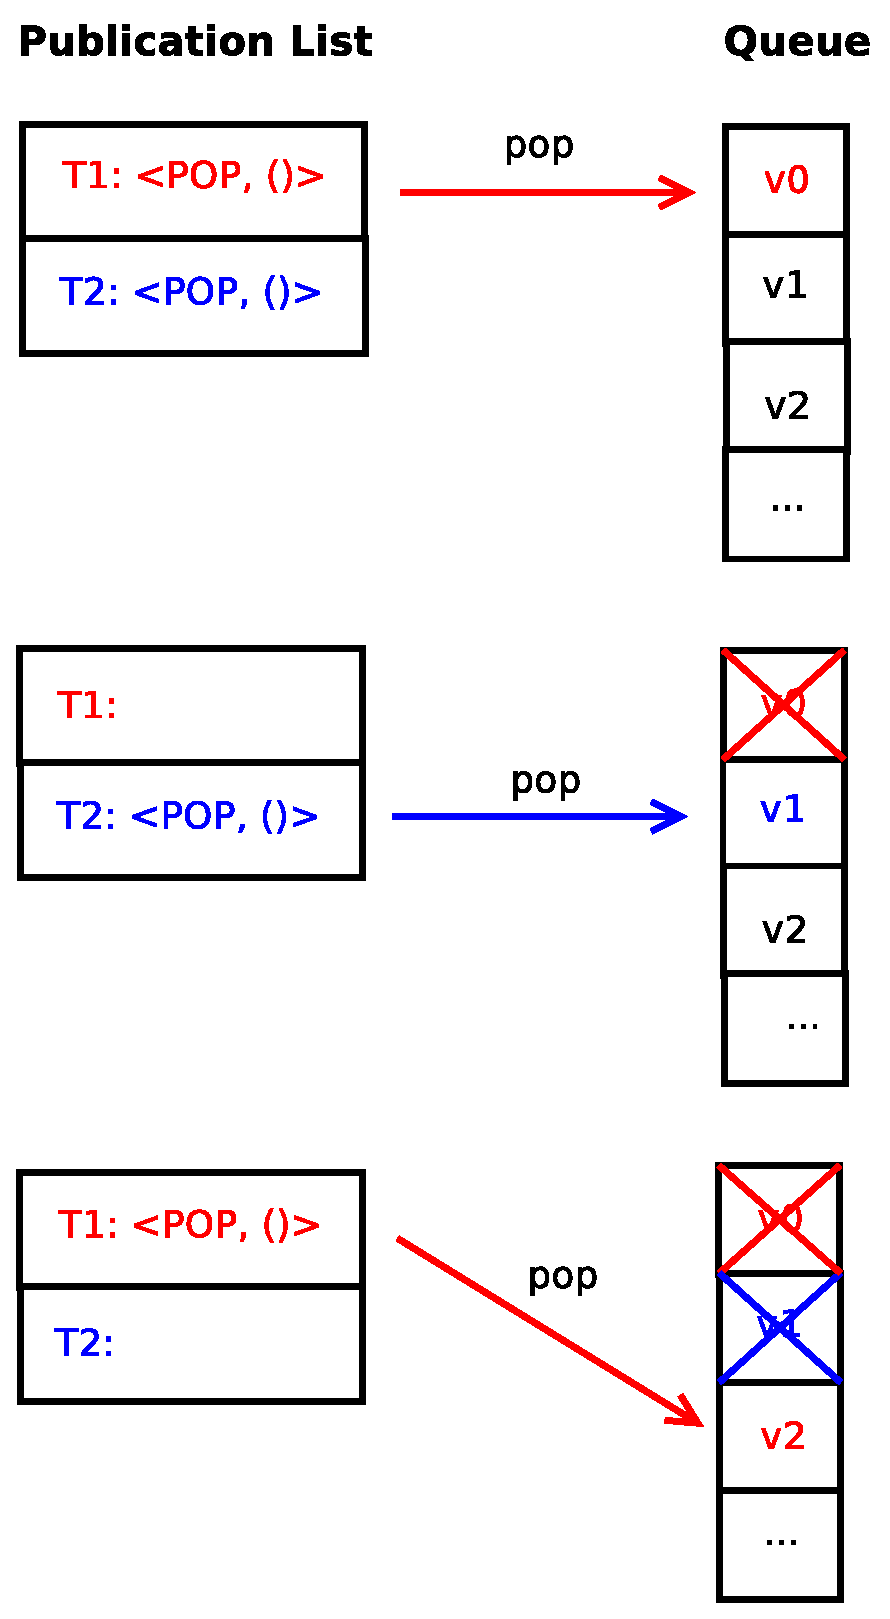
\includegraphics[width=0.45\textwidth]{fcqueue_publist}
    \caption[Invalid interleaving of pop requests in the flat combining queue]{This sequence of operations applied to the queue is a possible interleaving that will cause both transactions T1 and T2 to abort. A transactional flat combining queue must ensure that all pops in one transaction are consecutive and are of the head of the queue. In this example, T1 performs two pops and T2 performs one pop. The combiner thread applies T1's first pop, then T2's pop, and finally T1's second pop. Because T1's pops are not popping consecutive values off the queue, T1 is an invalid transaction, and must abort when it commits (not shown). When T1 aborts, the head ($v0$) of the queue is restored. T2 now becomes an invalid transaction because it popped a value that was not the head of the queue.}
\label{fig:fcqueue_publist}
\end{figure}

We now describe the new algorithms for push and pop.  We change the types of requests a thread can publish to its record on the publication list. Recall that the original flat combining queue supports two requests: \texttt{<PUSH, value>} and \texttt{<POP, ()>}. The transactional queue supports the follow requests:
\begin{itemize}
    \item \texttt{<PUSH, list>} : push a list of values onto the queue
    \item \texttt{<MARK\_POP, thread\_id>} : mark a value in the queue as ``to be popped'' by this \texttt{thread\_id}
    \item \texttt{<DEQ, thread\_id>} : dequeue all values in the queue that are marked ``to be popped'' by this \texttt{thread\_id}
    \item \texttt{<EMPTY?, thread\_id>} : check if the queue, after popping all items marked by this \texttt{thread\_id}, is empty
    \item \texttt{<CLEANUP, thread\_id>} : unmark all values that are marked with this \texttt{thread\_id}
\end{itemize}

As with the T-QueueO and T-QueueP, a push within a transaction adds to an internal \texttt{write\_list\_item}. At commit time, the thread will post a \texttt{<PUSH, list>} request with the \texttt{write\_list} passed as the argument.

A pop is implemented with a pessimistic approach. Performing a pop within a transaction invokes the \texttt{<MARK\_POP, thread\_id>} request. The combiner thread, upon seeing a \texttt{MARK\_POP} request, looks at the first value at the head of the queue. If this value is marked with another thread's \texttt{thread\_id}, the combiner thread returns \texttt{<ABORT>} to the calling thread. This scenario is shown in Figure~\ref{fig:fcqueue_abort1}.

\begin{figure}[t]
\centering
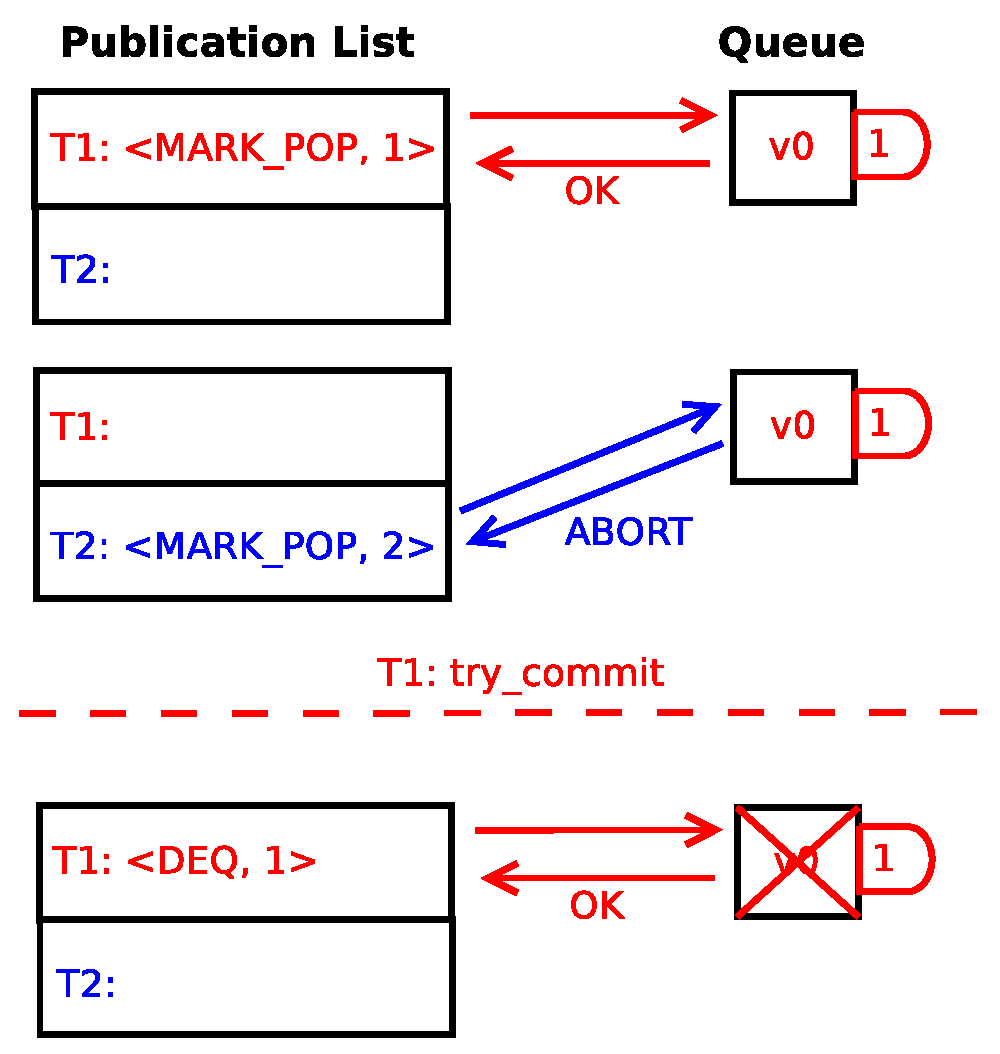
\includegraphics[width=0.45\textwidth]{fcqueue_abort1}
    \caption[Abort when performing conflicting pop requests]{T1 and T2 both attempt to mark the head of the queue with their \texttt{thread\_id}. T1's request is applied first, and marks the value $v0$ with the \texttt{thread\_id} 1. The combiner thread attempts to apply T2's request and sees T1's \texttt{thread\_id} marking the head of the queue. It then signals T2 to abort.}
\label{fig:fcqueue_abort1}
\end{figure}

If the value is not marked, the combiner thread marks the value with the caller's \texttt{thread\_id} and returns \texttt{<OK>}. Note that in this scenario, no other thread will be able to mark values in the queue until the calling thread commits or aborts; other threads will abort when seeing the head value marked by the calling thread's \texttt{thread\_id}. 

If the value is neither marked by another thread nor unmarked, then the value must already be marked with this thread's \texttt{thread\_id}, and the combiner thread iterates sequentially through the queue values until it reaches a value not marked by the calling thread's \texttt{thread\_id}. It then marks the value with the caller's \texttt{thread\_id} and returns \texttt{<OK>}. Upon receiving the response, the calling thread adds a write to a \texttt{pop\_item} to tell the thread to post a \texttt{<DEQ, thread\_id>} request at commit time. This request will tell the combiner thread to actually remove the popped value from the queue. This procedure is shown in Figure~\ref{fcqueue_deq}.

\begin{figure}[t]
\centering
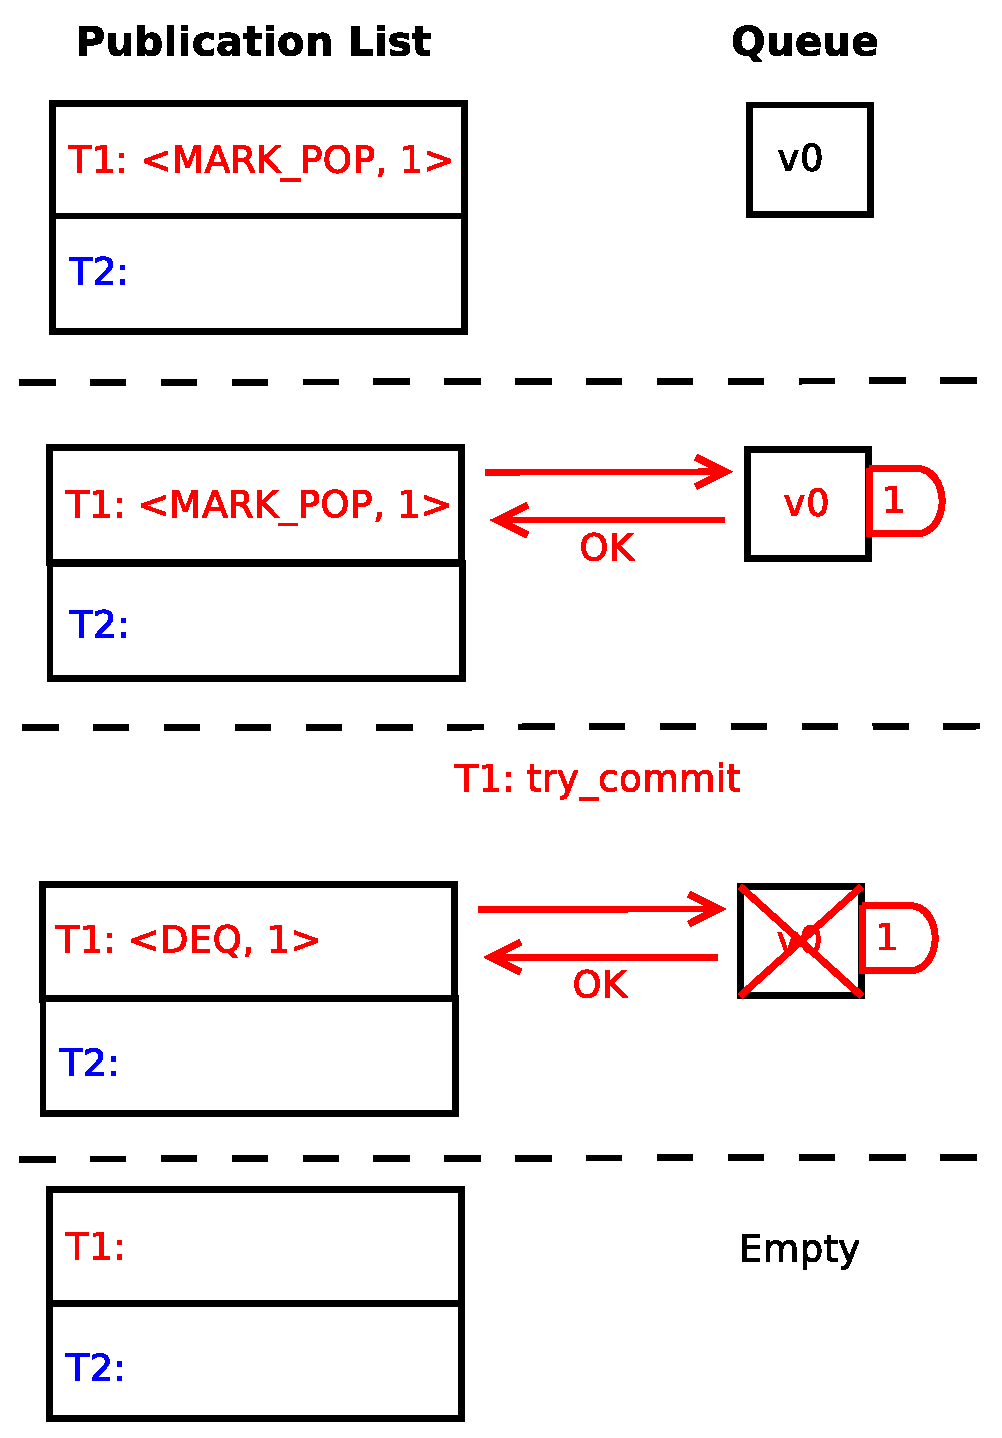
\includegraphics[width=0.45\textwidth]{fcqueue_deq}
    \caption[Transactional flat combining pop request execution]{T1 performs a pop by sending a \texttt{MARK\_POP} request, and marks the value in the queue with its \texttt{thread\_id} 1. At commit time, T1 actually performs the pop by sending a \texttt{DEQ} request.} 
\label{fig:fcqueue_deq}
\end{figure}

If the queue is empty, or all values are marked with the caller's \texttt{thread\_id}, the combiner thread will return \texttt{<EMPTY>}, which is remembered by the calling thread. An \texttt{<EMPTY>} response requires that the size of the queue be checked at commit time. If the calling thread has previously performed a push in the same transaction, the transaction performs \emph{read-my-writes} and removes the head of the \texttt{write\_list}; in this case, the transactional pop returns true. Otherwise, the pop returns false.

The \texttt{<EMPTY?, thread\_id>} request is posted at commit time when a thread tries to commit a transaction that observed an empty queue at some point in its execution. This happens when the thread receives an \texttt{<EMPTY>} response to a \texttt{<MARK\_POP>} request during the transaction. If \texttt{[<EMPTY?, thread\_id> == true]}, this implies that the queue state is currently empty.
The thread therefore knows that no other thread has pushed onto the queue since the time it saw an empty queue while performing a \texttt{<MARK\_POP>}, and it can safely commit the transaction. If \texttt{[<EMPTY?, thread\_id> == false]}, the queue is no longer empty---another thread has pushed items onto the queue---and this thread's \texttt{<MARK\_POP>} result is invalid. The transaction must therefore abort. This scenario is shown in Figure~\ref{fig:fcqueue_abort2}.

\begin{figure}[H]
\centering
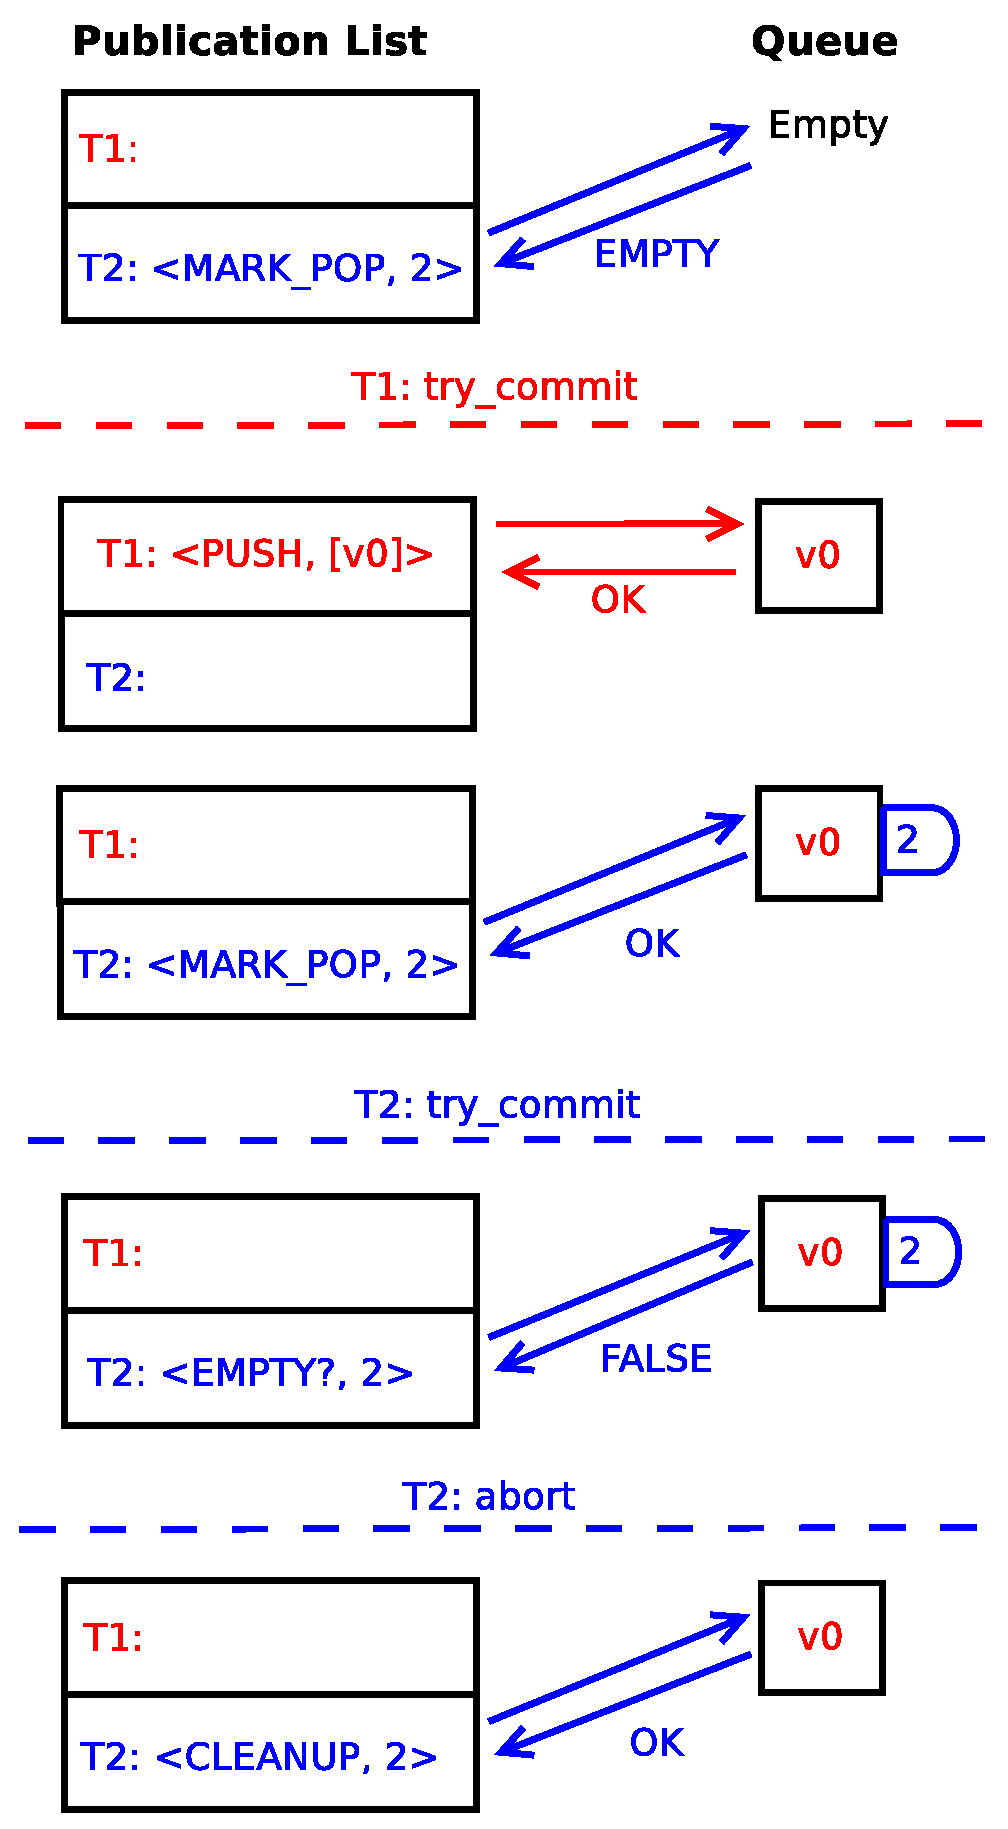
\includegraphics[width=0.45\textwidth]{fcqueue_abort2}
    \caption[Abort and cleanup when checking the empty status of the queue]{This sequence shows how a transaction can abort when checking \texttt{<EMPTY?>} in the transactional flat combining queue. T2 tries to pop from an empty queue, and sees the queue is empty. This means that when T2 commits, T2 will have to check if the queue is empty. T1 commits its transaction and pushes $v0$ onto the queue (recall that a push only executes at commit time). T2 then tries to pop another value off the queue and sees $v0$, marking it with its \texttt{thread\_id} 2. T2 tries to commit, but observes that the queue is no longer empty: T2 must abort. When T2 aborts, it must clean up any markers it left in the queue.}
\label{fig:fcqueue_abort2}
\end{figure}

If a thread ever sees an empty queue when executing a pop \emph{and} subsequently performs a push within the same transaction, the thread must prevent another transaction from committing between the time of the empty check and the installation of its pushed value. This requires adding what is essentially a lock of the tail of the queue. This is implemented via additional machinery in the combiner thread code, which signals whether or not a transaction has locked the queue and prevents any other thread's pushes from being installed until the ``lock'' is released.

The \texttt{<CLEANUP, thread\_id>} request is posted when a thread aborts a transaction and must unmark any items in the queue that it had marked as pending pops. The combiner thread iterates through the queue from the head and unmarks any items with the \texttt{thread\_id}. An example of this is shown in FIgure~\ref{fig:fcqueue_abort2}.

\section{Evaluation}

\subsection{Microbenchmarks}
\label{q_microbenchmarks}

We evaluate all the queue implementations on a set of microbenchmarks to determine their scalability and performance. The controlled nature of these microbenchmarks allows us to compare particular aspects of each algorithm, such as transactional overhead introduced by STO. All experiments are run on a 100GB DRAM machine with two 6-core Intel Xeon X5690 processors clocked at 3.47GHz. Hyperthreading is enabled in each processor, resulting in 24 available logical cores. The machine runs a 64-bit Linux 3.2.0 operating system, and all benchmarks and STO data structures are compiled with \texttt{g++-5.3}. In all tests, threads are pinned to cores, with at most one thread per logical core.
In all graphs, we show the median of 5 consecutive runs with the minimum and maximum performance results represented as error bars.

\subsubsection{Parameters}

\emph{Value Types}. Each queue benchmark uses randomly chosen integers because the benchmarks do not manipulate the push or popped values and the queue algorithms are agnostic to the actual values being placed in the queue.

\emph{Initial Queue Size}. We run our tests with varying numbers of initial entries in the queue. This affects how often the structure becomes empty, which can cause aborts and additional overhead (as described in the algorithms above). It also affects the number of cache lines accessed: a near-empty queue will never require iterating over values contained in more than one cache line.

\emph{Operations per transaction}. We set the number of operations per transaction to 1 (i.e., the transactions are singleton transactions). By keeping a transaction as short as possible, we maximize the impact of any fixed per-transaction overhead. However, we also minimize the performance hit from the additional transactional overhead required to maintain and commit larger read- or write-sets: running multiple-operation transactions requires multiple-item support in read- and write-sets, creates scenarios of read-my-writes, and increases the number of aborts and retries, all of which incur additional overhead. 
Because most highly-concurrent data structures provide guarantees equivalent to those of singleton transactions, we use singleton transactions when comparing transactional and non-transactional data structures.
Note that our data structure implementations can correctly handle multiple-operation transactions: we simply benchmark them with singleton transactions to compare performance.

\subsubsection{Tests}
    \emph{2-Thread Push-Pop Test}. This test has one thread that performs only pushes and another thread that performs only pops (a traditional ``producer-consumer'' model). Each thread performs 10 million transactions. Unless the queue is empty, the two threads should never be modifying the same part of the data structure and will never conflict, leading to an abort rate that should be near 0. We use this test to measure the speed of push/pops on the queue under low or no contention. We expect that our transactional queues should perform just as well as the highly-concurrent queues, if not better: while highly-concurrent, non-transactional algorithms are optimized for multi-threaded access, our simpler implementation should be just as fast with low contention and low abort rates.

\emph{Multi-Thread Singletons Test}.
    In this test, a thread randomly selects an operation (push or pop) to perform within each transaction. This keeps the queue at approximately the same size as its initial size during the test. Each thread performs 10 million transactions. We run this test with different initial queue sizes and different numbers of threads, with each thread performing singleton transactions. Altering the number of threads allows us to benchmark performance under variable amounts of contention. We expect that T-QueueO and T-QueueP queues will perform significantly worse once the number of threads is increased, and that these naive synchronization algorithms will underperform synchronization algorithms optimized for contentious situations.

\subsection{Overview of Results}

We discuss our results by first presenting an overview of our conclusions, and then explaining each in more detail by proposing a sequence of five hypotheses, which we test using the benchmarks described above. For each hypothesis, we use our benchmark results to formulate a conclusion that either refutes or supports the hypothesis.
We provide a few figures that highlight our results; full results (including abort rates) can be found in Appendix~\ref{app:queues}. 

Our results demonstrate the following:
\begin{itemize}
    \item Performance improves when implementing contentious operations with a pessimistic, rather than optimistic, approach.
    \item Fixed overhead from bookkeeping STO wrapper calls is negligible.
    \item The flat combining technique is a highly effective synchronization technique for queues, and the flat combining, non-transactional queue outperforms all transactional and concurrent queues.
    \item Performance of the transactional flat combining queue underperforms all transactional queues. The performance loss comes from the greater number and greater complexity of flat combining calls that are necessary to convert the non-transactional flat combining queue to a transactional one.
\end{itemize}

\subsection[Hypothesis 1]{Hypothesis 1}
\subsubsection{Using a pessimistic algorithm for pop achieves better performance than using an optimistic algorithm (Supported).}
\begin{figure}[ht!]
    \centering
	\begin{minipage}{0.75\textwidth}
        \boxed{\includegraphics[width=\textwidth]{fcqueues/stoQ:PushPop.png}}
        \caption*{Push-Pop Test (2 threads)}
        \vspace{12pt}
	\end{minipage}
	\begin{minipage}{0.75\textwidth}
        \boxed{\includegraphics[width=\textwidth]{fcqueues/stoQ:RandSingleOps10000.png}}
        \caption*{Multi-Thread Singletons Test}
	\end{minipage}
    \caption{T-QueueO vs. T-QueueP Performance}
    \label{fig:stoqs}
\end{figure}


We test this hypothesis by comparing the performance of T-QueueO and T-QueueP queue. These two queues differ only in that a thread running on T-QueueP queue locks the queue immediately when it performs a transactional pop, therefore pessimistically assuming that any other thread accessing the queue will cause a conflict with its pop operation.

The comparative performance of T-QueueO and T-QueueP (Figure~\ref{fig:stoqs}) demonstrates that using a pessimistic technique for transactional pop execution is more effective than an optimistic one. 
T-QueueP performs slightly better than T-QueueO on the Multi-Thread Singletons Test. This is likely due to T-QueueP's lower abort rate (1/3 that of T-QueueO): a pop in T-QueueP locks the queue and prevents any other thread from observing an inconsistent state. The T-QueueO allows threads to observe inconsistent state (i.e., execute a pop of a head that is about to be popped by another thread); this causes aborts at execution and commit time.
This result supports that a pessimistic approach to contentious operations such as pop benefits performance.

On the Push-Pop Test, T-QueueP's performance is double that of T-QueueO's performance. This result is initially surprising, because the Push-Pop Test is a low-contention test (the abort rates, as expected, are near 0, with aborts only occurring because the threads spin too long while acquiring locks). We therefore should expect that T-QueueP performs approximately equal to T-QueueO. However, this is clearly not the case.

Our results for the Push-Pop Test can be explained by the number of pops successfully completed by the pop-only thread at the time that the push-only thread has completed 10 million transactions and exits. The percentage of pops completed at the time 10 million pushes have completed are shown in Table~\ref{tab:sto_pop_push_ratio}.
We see that for both queues, the push-only thread completes its 10 million transactions much faster than the pop-only thread. However, T-QueueP's push-only thread beats the pop-only thread by a greater margin than does T-QueueO's push-only thread: T-QueueP's results show that only 28\% of the pops have completed by the time the push-only thread exits, while T-QueueO's results show that approximately 64\% of the pops have completed.

\begin{table}[t]
        \centering
    \begin{tabular}{|cc|}
        \hline
        Queue & Pops:Pushes\\
        \hline
            T-QueueO & 0.64\\
            T-QueueP & 0.28\\
        \hline
    \end{tabular}
    \caption{T-QueueO vs.\ T-QueueP Push-Pop Test Performance: Number of pops completed by the pop-only thread when the push-only thread has completed 10M pushes.}
    \label{tab:sto_pop_push_ratio}
\end{table}

We conclude that the modified algorithm for T-QueueP allows a push to execute much faster than a pop, and that this is because T-QueueP uses only one queue version as a global queue lock. Both a push and pop contend on this lock in order to install an operation; the push-only thread can potentially ``starve'' the pop-only thread by continuously succeeding in acquiring the lock.
T-QueueO, on the other hand, uses two versions (head and tail versions), and each thread acquires only one of these locks when performing an operation.
T-QueueP therefore achieves much better overall performance because the threads run in nearly a sequential fashion.
Single-thread execution on the queue results in better cache line performance (there can never be cache line bounces, because only one thread accesses the queue). Furthermore, there is zero contention on the queue locks. 
We note that T-QueueP's execution pattern also has the fortunate side effect of decreasing the probability that the queue becomes empty, since a greater number of pushes complete for every pop operation that completes.

While the result of the Push-Pop test is likely caused by the shared lock used by T-QueueP's push and pop operations, instead of T-QueueP's pessimistic pop execution, our results from the Multi-Thread Singletons Test do support our hypothesis. They indicate that a pessimistic approach does reduce the abort rate and lead to slightly better performance when two threads are both attempting to perform pops.

\vspace{12pt}
\noindent\fbox{\begin{minipage}{\textwidth}
    \textbf{SUPPORTED}: T-QueueP outperforms T-QueueO, indicating that a pessimistic approach is more appropriate for contentious operations such as pop.
\end{minipage}}


\subsection{Hypothesis 2}
\subsubsection{Hypothesis 2: Under low contention, a transactional queue with a naive concurrent algorithm performs reasonably well compared to the best concurrent, non-transactional queue algorithms (Supported).}

\begin{figure}[ht!]
    \centering
	\begin{minipage}{0.75\textwidth}
        \boxed{\includegraphics[width=\textwidth]{concurrent/allQ:PushPop.png}}
	\end{minipage}
    \caption{Push-Pop Test (2 threads): Non-transactional, concurrent queue performance compared to transactional queue performance}
    \label{fig:ntqs_pp}
\end{figure}

We benchmark a set of the best-performing highly-concurrent queue algorithms against our transactional queue implementations, T-QueueO and T-QueueP, using our low-contention test (the 2-Thread Push-Pop test) that is also optimized for a low abort rate. This acts as a best-case scenario for T-QueueO and T-QueueP algorithms. Selected results are shown in Figure~\ref{fig:ntqs_pp}.

Our implementation of the non-transactional flat combining queue, which we call NT-FCQueue, uses the flat combining queue implemented by the authors of the flat combining paper~\cite{flatcombining} (with minor modifications to remove memory leaks). Our implementations of the other highly-concurrent queues are taken from the open source Concurrent Data Structures (CDS) library implementations~\cite{libcds}. 

All concurrent, non-transactional queues achieve approximately equal performance on the Push-Pop Test besides NT-FCQueue, Segmented Queue~\cite{queue4}, and TsigasCycle Queue~\cite{queue5}. 
The T-QueueP outperforms all queues by at least 150\% on the 2-thread Push-Pop test. This is, as we discussed earlier, likely caused by T-QueueP's near-sequential execution on this test. We see in Table~\ref{tab:push_pop_ratio} that the pop-only threads of most queues complete more than 50\% of the 10 million pops before the push-only thread exits.
We also observe that NT-FCQueue is the only queue in which 10 million pops complete faster than 10 million pushes (the ratio is closest to one pop operation performed per push operation). This may explain its poor performance on the Push-Pop test as compared to the other queues.

\begin{table}[t]
        \centering
    \begin{tabular}{|cc|}
        \hline
        Queue & Pops:Pushes\\
        \hline
            T-QueueO & 0.64\\
            T-QueueP & 0.28\\
            NT-FCQueue & 1.10\\
            Basket & 0.42\\
            Moir & 0.62\\
            Michael-Scott& 0.54\\
            Optimistic & 0.50\\
            Read-Write & 0.84\\
            Segmented & 0.50\\
            TsigasCycle & 0.52\\
        \hline
    \end{tabular}
    \caption{Non-transactional Queues vs.\ T-QueueO and T-QueueP Push-Pop Test Performance: Ratio of completed pops to completed pushes.}
    \label{tab:push_pop_ratio}
\end{table}

Regardless of the difference in speed between the push-only and pop-only threads, we see that our naive algorithms perform as well as the majority of concurrent algorithms on this test: T-QueueO performs equally as well as any non-transactional queue. The Push-Pop Test is designed for low abort rates and minimal transactional overhead from tracking items in read- and write-sets. This allows the test to simply measure how fast the data structure can handle pushes and pops. It is unsurprising that, on this test, a simple synchronization strategy can outperform the majority of highly-concurrent algorithms which are optimized for scalability. 

This demonstrates that a simple implementation of a naive algorithm can consistently outperform more complex concurrent queue implementations, even when implemented using STO. The overhead added from STO does not inherently cripple performance---our transactional data structures can compete with several highly-concurrent, non-transactional data structures in particular cases. 

\vspace{12pt}
\noindent\fbox{\begin{minipage}{\textwidth}
    \textbf{SUPPORTED}: T-QueueP and T-QueueO outperform or achieve equal performance to all concurrent, non-transactional queues on the 2-Thread Push-Pop Test. This indicates that a simple concurrent algorithm in a transactional setting can perform well under optimal circumstances.
\end{minipage}}


\newpage
\subsection{Hypothesis 3}
\subsubsection{The flat combining algorithm is the most promising concurrent queue algorithm to integrate with STO (Supported).}
\label{eval:hypo3}

\begin{figure}[ht!]
    \centering
   	\begin{minipage}{0.75\textwidth}
        \boxed{\includegraphics[width=\textwidth]{concurrent/allQ:RandSingleOps10000.png}}
        \caption*{Multi-Thread Singletons Test}
	\end{minipage}
    \caption{Multi-Thread Singletons Test: Non-transactional, concurrent queue performance compared to transactional queue performance}
    \label{fig:ntqs}
\end{figure}

We run the same set of highly-concurrent queues from the previous hypothesis on the Multi-Thread Singletons Test, which provides a more realistic example of high-contention workloads that a queue may experience. We investigate how different concurrent, non-transactional algorithms perform in high-contention situations compared to the transactional T-QueueP, and look for the most scalable and performant high-concurrency queue that outperforms T-QueueP to integrate with STO. Selected results are shown in Figure~\ref{fig:ntqs}.

On this test, NT-FCQueue achieves performance over 2.5$\times$ greater than any other concurrent, non-transactional queue as the number of threads increases above 2. The Multi-Thread Singletons Test highlights the performance benefits of the flat combining queue: as contention increases, the flat combining queue reaches performance approximately double that of T-QueueP. In addition, the flat combining queue is the only queue that scales. All the other highly-concurrent algorithms perform worse than T-QueueP, regardless of the number of threads accessing the queue or the initial queue size. 
Although an increase in the duration of a transaction and number of operations per transaction causes T-QueueP to perform far worse than other concurrent queues, our results demonstrate that a simple synchronization algorithm can achieve equal performance to more complex synchronization algorithms on our benchmarks.\footnote{We rely on the specific libcds~\cite{libcds} implementation of these concurrent, non-transactional data structures, which may not be the most optimized versions of these data structures. However, the performance of these implementations on our tests matches their performance in other research evaluating these data structures~\cite{queue1, queue3}.}

A comparison with NT-FCQueue indicates that the concurrent queue algorithms in T-QueueO and T-QueueP are certainly not optimal for performance in a non-transactional setting.
Given these results, as well as the algorithmic benefits of the flat combining technique described in Section~\ref{fcqueuent}, we choose the flat combining queue to integrate with STO.

\vspace{12pt}
\noindent\fbox{\begin{minipage}{\textwidth}
    \textbf{SUPPORTED}: NT-FCQueue significantly outperforms all highly-concurrent, non-transactional queues \emph{and} T-QueueP on the Multi-Thread Singletons Test, indicating that flat combining may be the most promising algorithm to integrate with STO to create a more performant and scalable transactional queue. 
\end{minipage}}

\subsection{Hypothesis 4}
\subsubsection{Overhead from general STO bookkeeping does not cripple performance of a highly-concurrent queue algorithm (Supported).}

\begin{figure}[ht!]
    \centering
	\begin{minipage}{0.75\textwidth}
        \boxed{\includegraphics[width=\textwidth]{fcqueues/ntQ:PushPop.png}}
        \caption*{Push-Pop Test (2 threads)}
        \vspace{12pt}
	\end{minipage}
   	\begin{minipage}{0.75\textwidth}
        \boxed{\includegraphics[width=\textwidth]{fcqueues/ntQ:RandSingleOps10000.png}}
        \caption*{Multi-Thread Singletons Test}
	\end{minipage}
        \caption{NT-FCQueue vs. NT-FCQueueWrapped Performance}
    \label{fig:wrappedqs}
\end{figure}

We create a version of NT-FCQueue, called NT-FCQueueWrapped, that invokes general STO bookkeeping calls. The relative performance of NT-FCQueueWrapped to NT-FCQueue indicates how much of the overhead added by the STO system is unavoidable (without modifying STO itself). 
Selected results are shown in Figure~\ref{fig:wrappedqs}.

The STO wrapper functions called by NT-FCQueueWrapped must be called by any user of the data structure in order for the data structure to perform the necessary bookkeeping to support transactions.
These two calls are \texttt{start\_transaction} and \texttt{try\_commit}, and allow a user to mark which operations should occur together in the same transaction. An example of how these calls are used are in Figure~\ref{fig:wrappers}. After invoking the \texttt{start\_transaction} call, the thread is able to collect items in its read- and write-sets. At the end of a transaction, the thread invokes the \texttt{try\_commit} call to run the commit protocol. The NT-FCQueueWrapped adds no items to the read- and write-sets after invoking \texttt{start\_transaction} and does nothing in its commit protocol. This means that NT-FCQueueWrapped incurs the minimum amount of overhead necessary to use STO and therefore represents the upper bound on the performance we can expect from a fully transactional flat combining queue (T-FCQueue). 

\begin{figure}[ht!]
\centering
\singlespace
\lstset{
	language=C++,
	basicstyle=\ttfamily\small,
	keywordstyle=\color{blue}\ttfamily,
	stringstyle=\color{red}\ttfamily,
	commentstyle=\color{green}\ttfamily,
	morekeywords={true, false},
}
	\begin{lstlisting}
                    Sto::start_transaction();
                    try {
                        do_queue_op(push, 1);
                        do_queue_op(pop, 0);
                        if (Sto::try_commit()) {
                            printf("committed");
                        }
                    } catch (Transaction::Abort e) {
                        printf("aborted");
                    }
	\end{lstlisting}
\caption{Example usage of STO wrapper calls}
\label{fig:wrappers}
\end{figure}

We see from our Multi-Thread Singletons Test that the STO wrapper calls can lead to a loss of performance ranging from 0\% at twenty threads to 30\% at four threads compared to the performance of the vanilla non-transactional flat combining queue. 
 With fewer threads accessing the queue, the proportion of overhead from the STO wrapper calls is greater because the overhead from synchronizing access to the queue is minimal. As the number of threads increases, the STO wrapper call overhead becomes negligible in comparison to the cost of synchronization.
NT-FCQueueWrapped retains most of NT-FCQueue's scalability, and the two queues perform equally well after the number of threads reaches approximately 14.

We also see an impact on performance of NT-FCQueue in the Push-Pop Test (performance drops by approximately 20\%). The push-only thread now beats the pop-only thread in NT-FCQueueWrapped, but the ratio is still close to one pop operation performed per push operation (Table~\ref{tab:nt_pop_push_ratio}). The performance impact likely comes form the overhead added by STO wrapper calls; this is expected, as we discussed before, because this constant overhead more significantly affects performance at low thread counts and low contention.

\begin{table}[ht!]
        \centering
    \begin{tabular}{|cc|}
        \hline
        Queue & Pops:Pushes\\
        \hline
            NT-FCQueue & 1.10\\
            NT-FCQueueWrapped & 0.94\\
        \hline
    \end{tabular}
    \caption{NT-FCQueue vs.\ NT-FCQueueWrapped Push-Pop Test Performance: Ratio of completed pops to completed pushes.}
    \label{tab:nt_pop_push_ratio}
\end{table}

Comparing NT-FCQueueWrapped and NT-FCQueue demonstrates that STO introduces unavoidable overhead that becomes negligible at high thread counts. Even with the wrapper calls, our results indicate it can still be possible to achieve performance up to nearly 2$\times$ greater at 20 threads than that of T-QueueP (the second-best performing queue).

\vspace{12pt}
\noindent\fbox{\begin{minipage}{\textwidth}
    \textbf{SUPPORTED}: Adding the calls to the general STO wrapper functions that are necessary for any data structure to support transactions does not cripple the performance of highly-concurrent queues such as NT-FCQueue, particularly at high thread counts.
\end{minipage}}

\subsection{Hypothesis 5}
\subsubsection{A transactional flat combining queue outperforms and scales better than a transactional queue with a naive concurrent algorithm (Not Supported).}
\label{eval:hypo5}

\begin{figure}[ht!]
    \centering
	\begin{minipage}{0.75\textwidth}
        \boxed{\includegraphics[width=\textwidth]{fcqueues/tQ:PushPop.png}}
        \caption*{Push-Pop Test (2 Threads)}
        \vspace{12pt}
	\end{minipage}
   	\begin{minipage}{0.75\textwidth}
        \boxed{\includegraphics[width=\textwidth]{fcqueues/tQ:RandSingleOps10000.png}}
        \caption*{Multi-Thread Singletons Test}
	\end{minipage}
        \caption{T-FCQueue Performance}
    \label{fig:tqs}
\end{figure}

We compare T-FCQueue against NT-FCQueueWrapped and T-QueueP to measure how the flat combining transactional approach described in Section~\ref{fcqueuet} performs. Selected results are shown in Figure~\ref{fig:tqs}.

In the Push-Pop Test (Figure~\ref{fig:tqs}), T-QueueP outperforms both flat combining variants. This is an unsurprising result given our results from the concurrent queues benchmark in Figure~\ref{fig:ntqs}, and the fact that T-FCQueue has a more equal ratio of pops to pushes than does T-QueueP (Table~\ref{tab:tfc_pop_push_ratio}). 

\begin{table}[t]
        \centering
    \begin{tabular}{|cc|}
        \hline
        Queue & Pops:Pushes\\
        \hline
            T-QueueP & 0.28\\
            NT-FCQueueWrapped & 0.94\\
            T-FCQueue & 0.57\\
        \hline
    \end{tabular}

    \caption{T-FCQueue Push-Pop Test Performance: Ratio of completed pops to completed pushes.}
    \label{tab:tfc_pop_push_ratio}
\end{table}

The Multi-Threaded Singletons Test (Figure~\ref{fig:tqs}) shows that T-QueueP performs approximately 2$\times$ better than T-FCQueue, regardless of initial queue size. Both queues do not scale, and the performance ratio remains constant regardless of the number of threads. The T-FCQueue also experiences abort rates around 5\%, which are $1.5$--$2\times$ the abort rates of T-QueueP.

\vspace{12pt}
\noindent\fbox{\begin{minipage}{\textwidth}
\textbf{NOT SUPPORTED}: The transactional flat combining queue does not outperform or scale better than other transactional queues using naive synchronization mechanisms. The T-FCQueue's poor performance compared to that of T-QueueP demonstrates that the flat combining algorithm performs poorly when modified to support transactions.
\end{minipage}}

\subsection{Conclusion}
Analysis with the \texttt{perf} tool indicates that the majority of T-FCQueue's overhead comes from spinning on the flat combining lock (acquired by the combiner thread) or waiting for a flat combining call to complete. In addition, the number of cache misses is over 4$\times$ greater than that of NT-FCQueue (see Figure~\ref{fig:qcm}). This overhead occurs for two reasons:
\begin{enumerate}
    \item \emph{Higher Quantity}: As described in Section~\ref{fcqueuet}, a thread must make multiple flat combining calls to perform a pop within a transaction (recall that a push only requires one flat combining call).
\item \emph{Higher Complexity}: each flat combining call requires executing instructions, which makes each operation request more expensive.
\end{enumerate}

We conclude that the flat combining technique, while perhaps near-optimal for a highly-concurrent data structure, is no better in a transactional setting than a naive synchronization technique such as that used in T-QueueO and T-QueueP. The flat combining algorithm must track the state of the queue during the transaction's lifetime to provide transactional guarantees (e.g., marking values in the queue or observing that the queue was empty when performing a pop). To do so requires both adding new flat combining calls and increasing the complexity of existing ones; these modifications cripple flat combining's performance.
In the next chapter, we formalize this argument using commutativity and claim that the flat combining technique fundamentally depends on operation commutativity present in only a non-transactional setting to achieve its high performance. 

\chapter{Commutativity and Scalability in Transactional Queue Specifications}
\label{commutativity}

This chapter describes the commutativity of our queue operations both in a non-transactional setting and in a transactional setting, and relates the amount of queue operation commutativity to queue implementation performance. For clarity, we refer to the queue operation interface shown in Figure~\ref{fig:q_interface} as the \emph{strong queue specification}; a transactional queue with this interface is the \emph{strong transactional queue}. We hypothesize that the strong queue specification cannot be implemented in a transactional setting in an efficient way due to the lack of operation commutativity in the strong queue specification. 
We follow this by proposing an alternative queue specification---the \emph{weak queue specification}---that allows for greater operation commutativity, and hypothesize that this alternative specification will allow for greater transactional queue scalability.

As a supporting example of our hypotheses, we examine the flat combining technique in detail and argue that the flat combining technique cannot implement the strong queue interface efficiently in a transactional setting. While the flat-combining technique is perhaps near-optimal for a highly-concurrent data structure, it performs no better than a naive synchronization technique in a transactional data structure. This is because the flat combining algorithm's high performance comes from exploiting the greater operation commutativity present in a non-transactional setting. The flat combining algorithm's optimizations must be heavily modified in order to support transactions, which leads to significant performance loss. 

We then implement a weak transactional flat combining queue---a flat combining queue with operations satisfying the weak queue specification---with the expectation that the flat combining technique can achieve scalable performance close to its performance in a non-transactional setting. Our experimental results illustrate that the greater commutativity of operations in the weak queue specification is essential for the flat combining technique to be effective in a transactional setting.

\section{History Terminology}

We introduce some terminology about histories and transactional histories that will be used in our discussion of operation commutativity.

\begin{defn}
    A \emph{history} is a sequence of \texttt{(thread, operation, result)} tuples that represent an interleaving of operations of all threads. Knowledge of both the history and initial conditions of a data structure leads to complete knowledge of the (high-level) end state of the structure.
\end{defn}

\begin{eg}
    \singlespacing   

    \begin{lstlisting}

    // Q.size() == 0 
    (T2, Q.push(a), ())
    (T1, Q.pop(), true)
    (T2, Q.push(a), ())
    (T1, Q.pop(), true)
    // Final State: Q.size() == 0 
    \end{lstlisting}
    \doublespacing
\end{eg}
\begin{defn}
    A \emph{transactional history} is a specific type of history in which the tuples represent an interleaving of operations of the threads' committed transactions. A transactional history includes \texttt{(thread, START\_TXN, ())} and \texttt{(thread, COMMIT\_TXN, commit\_result)} operation tuples that represent the time the thread starts and commits the transaction. \texttt{commit\_result} represents the observable effects of the installation procedure at commit time.

\begin{eg}
    \singlespacing   

    \begin{lstlisting}

    // Q.size() == 0 
    (T1, START_TXN, ())
    (T2, START_TXN, ())
    (T2, Q.push(a), ())
    (T1, Q.pop(), true)
    (T2, Q.push(a), ())
    (T1, Q.pop(), true)
    (T1, COMMIT_TXN, ())
    (T2, COMMIT_TXN, ())
    // Final State: Q.size() == 0 
    \end{lstlisting}
    \doublespacing
\end{eg}

\end{defn}

\begin{defn}
    A history $H'$ is \emph{consistent} with $H$ if:
    \begin{enumerate}
        \item $H'$ contains the same tuples as $H$: the same operations were executed with the same return values for all operations within the transactions.
        \item The order of a single thread's calls in $H'$ remains consistent with the thread's order of calls in $H$.
    \end{enumerate}
\end{defn}

\begin{defn}
    A transactional history $H$ is \emph{serial} if all tuples are grouped by transaction: if $i\le j\le k$ and $H_i$ and $H_k$ are from the same transaction, then $H_j$ is also from that transaction. This means the tuples form a serial transaction order.
\end{defn}
\begin{defn}
    A transactional history $H$ is \emph{serializable} if there exists a serial history $H'$ s.t. $H'$ is consistent with $H$.

\end{defn}

\begin{eg}
    $H$ is a serializable transactional history whose corresponding serial execution is $H'$. $H''$ represents a serial transactional history, but is inconsistent with $H$ because its pop operations return different results.
\begin{figure}[H]
\singlespacing   
   \begin{tabular}{c|c|c}
H & H' & H''\\
\hline
\begin{lstlisting}
// Q.size() == 0 
(T1, START_TXN, ())
(T2, START_TXN, ())
(T2, Q.push(a), ())
(T1, Q.pop(), true)
(T2, Q.push(a), ())
(T1, Q.pop(), true)
(T1, COMMIT_TXN, ())
(T2, COMMIT_TXN, ())
\end{lstlisting} & 
\begin{lstlisting}
// Q.size() == 0 
(T2, START_TXN)
(T2, Q.push(a), ())
(T2, Q.push(a), ())
(T2, COMMIT_TXN)
(T1, START_TXN)
(T1, Q.pop(), true)
(T1, Q.pop(), true)
(T1, COMMIT_TXN)
\end{lstlisting} &
\begin{lstlisting}
// Q.size() == 0 
(T1, START_TXN)
(T1, Q.pop(), false)
(T1, Q.pop(), false)
(T1, COMMIT_TXN)
(T2, START_TXN)
(T2, Q.push(a), ())
(T2, Q.push(a), ()) 
(T2, COMMIT_TXN)
\end{lstlisting}
\end{tabular}
\end{figure}
\end{eg}

\begin{defn}
A transactional history is \emph{linearizable} if all transactions appears to occur instantaneously between their start time and their commit time: if transaction $T1$ commits before transaction $T2$, then $T1$ must appear before $T2$ in the serial history~\cite{harristm}.
\end{defn}

\begin{defn}
    A transactional history $H$ is \emph{strictly serializable}, or \emph{valid}, if it is both serializable and linearizable. Any data structure implemented in a transactional setting requires strictly serializable transactional histories.
\end{defn}

\begin{eg}
$H$ is a serializable, but not linearizable transactional history. This is because $T2$ should have observed the pushes committed by $T1$. We can find a serial ordering of $H$, shown in $H'$, but $H'$ violates the rule that the serial order of transactions corresponds to the real time order of the transactions' commits.
    
\begin{figure}[H]
    \centering
\singlespacing   
    \begin{tabular}{c|c}
H & H'\\
\hline
\begin{lstlisting}
// Q empty                          
(T1, START_TXN)
(T1, Q.push(a), ())                
(T1, Q.push(a), ())               
(T1, Q.pop(), true)
(T1, COMMIT_TXN)
(T2, START_TXN)
(T2, Q.pop(), false)
(T2, COMMIT_TXN)
\end{lstlisting} & 
\begin{lstlisting}
// Q empty
(T2, START_TXN)
(T2, Q.pop(), false)
(T2, COMMIT_TXN)
(T1, START_TXN)
(T1, Q.push(a), ())                       
(T1, Q.push(a), ())
(T1, Q.pop(), true)
(T1, COMMIT_TXN)
\end{lstlisting}
    \end{tabular}
\end{figure}
\end{eg}

\section{The Relationship of Commutativity and Scalability}

The \emph{scalable commutativity rule}, formally defined by Clements et al.~\cite{scrule}, asserts that whenever interface operations \emph{commute}, there exists an implementation of the interface that scales.
Operations \emph{commute} in a particular interface when there is no way to distinguish their execution order: exchanging the order of the operations in the history does not modify the return values of the operations seen by each thread.

\subsection{Commutativity of the Strong Queue Specification} 

In a non-transactional setting, we consider histories in which the only operations are push and pop (i.e., the histories are not transactional). Given the strong queue specification (Figure~\ref{fig:q_interface}) in which push returns \texttt{void} and pop returns \texttt{bool}, we determine the commutativity of these operations by examining if exchanging the order in which the operations appear in the history changes the operations' return values. We show operations that do not commute in Table~\ref{tab:strongq_commute}.
Based on this commutativity analysis, we note that a pop operation does not commute with a push operation when the queue is empty, or another pop operation when the queue is near empty. By the scalable commutativity rule, this means that there is no concurrent queue implementation for pop that scales in these particular scenarios. A push operation commutes with all operations because it returns \texttt{void}, and has a scalable implementation in all scenarios.

\begin{table}[t]
    \singlespace
    \centering
    \begin{tabular}{|c|l|l|}
        \hline
        Operations & \multicolumn{1}{c}{H} & \multicolumn{1}{|c|}{H'} \\
        \hline
    
        push vs. pop &
\begin{lstlisting}
// Q empty
(T, Q.push(a), ())                       
(T, Q.pop(), true)
\end{lstlisting} &
\begin{lstlisting}
// Q empty
(T, Q.pop(), false)
(T, Q.push(a), ())                       
\end{lstlisting}\\
\hline

    pop vs. pop &
\begin{lstlisting}
// Q.size() = 1
(T1, Q.pop(), true)
(T2, Q.pop(), false)                       
\end{lstlisting} &
\begin{lstlisting}
// Q.size() = 1
(T2, Q.pop(), true)
(T1, Q.pop(), false)                       
\end{lstlisting}\\
    \hline

    \end{tabular}
    \caption[Strong queue operations that do not commute]{Strong queue operations that do not commute. H is the original history; H' is the history with the order of the two operations exchanged. In the push vs pop scenario, note that any thread may have performed the operations, and the operations will still not commute.}
    \label{tab:strongq_commute}
    \end{table}

We reason about commutativity of a queue implemented in a transactional setting using transactional histories, which include \texttt{START\_TXN} and \texttt{COMMIT\_TXN} operations. A transactional setting calls for strict serializability of the transactional history, which by definition entails serializability (i.e., that tuples in histories be grouped by transaction). This adds an additional level of commutativity, namely commutativity between transactions.

Because a valid transactional history is strictly serializable, we can find a corresponding serial history for every valid transactional history. This means that operations belonging to the same transaction must occur in a group in the history. To reason about transaction commutativity, we have a parallel notion to exchanging operations in the history to detect whether two operations commutate:  we exchange \emph{groups} of operations in a \texttt{START\_TXN} and \texttt{COMMIT\_TXN} block of a serial history, and detect whether there is any observable change in the return values within the exchanged transactions. Because the occurrence of each transaction in the serial transactional history can be uniquely identified by its \texttt{COMMIT\_TXN} tuple: if exchanging the positions of two transactions does not commute in a particular scenario, we can say that the two \texttt{COMMIT\_TXN} operations do not commute in that scenario.

We also must now consider when \texttt{COMMIT\_TXN} operations do not commute. Note that when transactions contain only one operation, then a lack of commutativity between two transactions is equivalent to saying that that the two operations do not commute (and vice versa). We provide a constructive approach to find all non-singleton transactions in the history whose lack of commutativity prevents their order from being exchanged. This approach works by extending the singleton operations transactions that do not commute---identified in Table~\ref{tab:strongq_commute}---as follows: 
\begin{itemize}
    \item Let transaction $T1$ perform some ordered set of operations $O_1$ and transaction $T2$ perform some ordered set of operations $O_2$. Let $H$ be a (serial) history in which $T1$ and $T2$ do not commute, and $H'$ be the history in which the order of $T1$ and $T2$ has been exchanged. Let $H_{new}$ and $H'_{new}$ be the histories when $T1$ or $T2$ is extended with new operations.
    \item Assume $T1$ and $T2$ do not commute: WLOG, let at least one of the return values of an operation in $O_1$ change when the order of $T1$ and $T2$ is exchanged in $H$. We know this happens only if exchanging the order of $T1$ and $T2$ causes a pop operation in $T1$ to observe an empty queue given one order, but not in another.
    \item We extend $T1$ with operations $O_3$ appended to $O_1$, where $O_3$ is some arbitrary set of operations. Then $T1$ performing $O_1 + O_3$ does not commute with $T2$. This is because we will have in $O_1 + O_3 + O_2$ in $H_{new}$, and $O_2 + O_1 + O_3$ in $H'_{new}$: the return values of $O_1$ in $O_1 + O_3 + O_2$ are the same as in $O_1 + O_2$, and the return values of $O_1$ in $O_2 + O_1 + O_3$ are the same as in $O_2 + O_1$.
    \item We extend $T1$ with operations $O_4$ added to the front of $O_1$. $O_4$ is an ordered set of operations such that at least one pop in $O_1$ observes an empty queue in $H_{new}$ or $H'_{new}$, and a nonempty queue in the other. Then $T1$ performing $O_4 + O_1$ does not commute with $T2$ by definition.
\end{itemize}

Conversely, we know that these arbitrarily large, non-commuting transactions that we find through our construction are the \emph{only} transactions that do not commute: 
\begin{itemize}
    \item Let transaction $T1$ perform some ordered set of operations $P$ and transaction $T2$ perform some ordered set of operations $Q$.
    \item We are given that $T1$ and $T2$ do not commute. WLOG, this means that we can find some $o \in P$ s.t. $o$'s return value changes when we exchange the order of $T'$ and $T''$ in the history, and $o$ is the first such operation (necessarily a pop) in $P$ s.t.\ this occurs.
    \item We deconstruct $O$ into the following ordered set: $O' + \{o\} + O''$. Let $\{o\}$ be $O_1$ from the construction above. 
        Let $O'$ be $O_4$: $O'$ satisfies the properties of $O_4$ specified above, because $o$ provides the witness for the pop in $O_1$ that observes an empty queue $H_{new}$ or $H'_{new}$ and a nonempty queue in the other. We can also find a witness for $O_3$, namely $O''$: because $O' + \{o\}$ does not commute with $T1$, our construction will generate $P = O' + \{o\} + O''$ as operations of a transaction $T1$ that does not commute with $T2$.
\end{itemize}

\begin{table}[t]
    \singlespace
    \centering
    \begin{tabular}{|c|l|l|}
        \hline
        Example & \multicolumn{1}{c}{H} & \multicolumn{1}{|c|}{H'} \\
        \hline
        1. & 
\begin{lstlisting}
// Q empty
(T1, START_TXN, ())                       
(T1, Q.pop(), false)                       
(T1, Q.push(a), ())                       
(T1, COMMIT_TXN, ())                       
(T2, START_TXN, ())                       
(T2, Q.pop(), true)                       
(T2, COMMIT_TXN, ())                       
\end{lstlisting} &
\begin{lstlisting}
// Q empty
(T2, START_TXN, ())                       
(T2, Q.pop(), false)                       
(T2, COMMIT_TXN, ())                       
(T1, START_TXN, ())                       
(T1, Q.pop(), false)                       
(T1, Q.push(a), ())                       
(T1, COMMIT_TXN, ())                       
\end{lstlisting}\\
\hline
    2. &
\begin{lstlisting}
// Q empty
(T1, START_TXN, ())                       
(T1, Q.push(a), ())                       
(T1, Q.pop(), true)                       
(T1, Q.push(a), ())                       
(T1, COMMIT_TXN, ())                       
(T2, START_TXN, ())                       
(T2, Q.pop(), (true))                       
(T2, Q.push(a), ())                       
(T2, COMMIT_TXN, ())                       
\end{lstlisting} &
\begin{lstlisting}
// Q empty
(T2, START_TXN, ())                       
(T2, Q.pop(), (false))                       
(T2, Q.push(a), ())                       
(T2, COMMIT_TXN, ())                       
(T1, START_TXN, ())                       
(T1, Q.push(a), ())                       
(T1, Q.pop(), true)                       
(T1, Q.push(a), ())                       
(T1, COMMIT_TXN, ())                       
\end{lstlisting}\\
    \hline
    
    \end{tabular}
    \caption[Examples of strong queue transactions that do not commute]{Examples of strong queue transactions that do not commute. For clarity, we show only the serial history corresponding to the original valid transactional history.
    H is the original serial history; H' is the history with the order of the two transactions exchanged.}
    \label{tab:txnal_strongq_commute}
    \end{table}

We provide some examples of larger transactions that fail to commute in Table~\ref{tab:strongq_commute}.

Based on this commutativity analysis, we note that, in addition to the non-commutativity of pop operations in particular scenarios involving empty, or near-empty queues, we now have a further lack of commutativity of transactions (identified by their \texttt{COMMIT\_TXN} operations) even in scenarios in which the queue may contain far more than one element. For example, even if a transaction starts with a relatively non-empty queue, a large transaction that performs several pops may reduce the queue to a near-empty state, and therefore contain a pop operation that observes the empty status of the queue. This transaction will likely \emph{not} commute with any other transaction performing a push or pop.  By the scalable commutativity rule, this means that there is no scalable queue implementation for a strong transactional queue whenever \texttt{COMMIT\_TXN} operations do not commute.

We hypothesize that any implementation of our strong queue specification in a transactional setting that must handle scenarios in which queues may become empty will not scale. A concurrent queue already lacks a scalable implementation for pop due to the high likelihood that a pop operation will not commute with any other operation when the queue nears empty. When this queue is put in a transactional setting, there is an even higher likelihood that two transactions will not commute, even if the queue contains more values. This prevents an efficient, scalable implementation of a strong transactional queue. In Section~\ref{wqueue}, we provide a counterexample, a transactional queue satisfying the \emph{weak queue specification}, and demonstrate how increased commutativity in this new specification allows for a scalable implementation.

\subsection{Strong Transactional Flat Combining Queue Performance}
The flat combining algorithm is an example of a queue algorithm that implements the strong queue interface and loses its effectiveness in a transactional setting. Recall that our results from testing Hypothesis 5 demonstrate that flat combining's effectiveness is lost in a transactional setting. Here, we argue that this is due to a decrease in the amount of commutativity in the transactional setting: in addition to non-commutative single operations (pops and pushes), transactions may not always commute.

Flat combining's fundamental principle is that requests posted to the publication list can be blindly applied to the queue in an arbitrary order. It handles the non-commutativity on the level of individual pop operations by synchronizing concurrent access to the queue with the combiner thread: only one thread is allowed to perform an operation on the queue at a time.\footnote{We note that flat combining is not a scalable implementation of pop (or push): the combiner thread's application of requests can only be as efficient as a sequential execution of all thread operations. As our results from testing Hypothesis 3 show, flat combining is nonetheless the most efficient of all concurrent queue algorithms evaluated.}
In a strong transactional queue, the flat combining algorithm must also correctly handle transactions that may not commute, which means synchronizing the \texttt{COMMIT\_TXN} operations of different transactions. This requires that the algorithm prevent operations within transactions from interleaving in the transactional history in a way that prevents the transactional history from being serialized. In other words, the order in which operations are applied becomes important.

We show all invalid interleavings of operations that will violate transactional guarantees (i.e., cause histories to be non-strictly serializable) in Table~\ref{tab:interleavings}.\footnote{We derive these following Schwarz's method~\cite{schwarz} that reasons about invalid histories using \emph{dependencies}. All operations performed by a transaction can be thought of in terms of reads and writes, and these operations create read-write, write-write, etc.\ dependency edges between two transactions. Schwartz asserts that invalid histories must necessarily include cycles in the dependency graph consisting of some number of read-write, write-read, or write-write edges.}
Preventing these interleavings requires adding complexity to each flat combining call (pop and push), as well as adding flat combining calls to check, undo, or install at commit time. We describe several methods to do so, and argue that these methods cannot be integrated with the flat combining algorithm without introducing overhead that reduces its performance to below that of the T-QueueO or T-QueueP. 

\begin{table}
    \centering
    \begin{tabular}{|c|l|}
        \hline
\multicolumn{2}{|c|}{Interleaving}\\
        \hline
1. & 
\begin{lstlisting}
(T1, Q.pop(), true/false)  
(T2, Q.pop(), true/false)       
(T1, Q.pop(), true/false)
\end{lstlisting} 
       \\ 
    \hline
        2. & 
\begin{lstlisting}
// Q.size() == 1  
(T1, Q.pop(), true) // Q empty  
(T2, Q.push(a), ())
(T1, Q.pop(), true)
\end{lstlisting} 
       \\ 
    \hline
        3. & 
\begin{lstlisting}
// Q.size() == 1  
(T1, Q.pop(), true)  // Q empty  
(T2, Q.pop(), false)
(T1, Q.push(a), ())
\end{lstlisting} 
\\
\hline
        4. &
\begin{lstlisting}
(T1, Q.push(a), ()) 
(T2, Q.push(a), ())
(T1, Q.push(a), ())
\end{lstlisting} 
\\
\hline
        5. &
\begin{lstlisting}
// Q.size() == 0 
(T1, Q.push(a), ())       
(T2, Q.pop(), true)  // Q empty
(T1, Q.pop(), false) 
\end{lstlisting} 
\\
    \hline
\end{tabular}
    \caption{Invalid operation interleavings in transactional histories.}
    \label{tab:interleavings}
\end{table}

A standard method for a transactional queue is to delay push operation execution, and to use a pessimistic or optimistic approach when encountering an empty queue.
To prevent interleavings 4 and 5, all pushes are delayed until commit time. These interleavings can occur only if $T1$'s first push is visible to $T2$ prior to $T1$'s commit. If we delay pushes until commit time, $T2$ will not detect the presence of a pushed item in the queue.

Because pop operations immediately return values that depend on the state of the queue (\texttt{false} if the queue is empty or \texttt{true} if the queue is nonempty), interleavings 1, 2, and 3 cannot be prevented by delaying pop operations until commit time. Instead, we can take one of two approaches. Let $T1$ be a transaction that has performed a pop.
\begin{enumerate}
    \item Optimistic: Abort $T1$ at commit time if $T2$ has committed an operation that would cause an invalid interleaving.
    \item Pessimistic: Prevent $T2$ from committing any operation until after $T1$ commits or aborts.
\end{enumerate}

The T-QueueO implements the optimistic method: checks of the tail version and the head version determine at commit time whether the empty status of the queue has been modified by another, already committed transaction. The T-QueueP implements the pessimistic approach, which locks the queue after a pop is performed and only releases the lock if the transaction commits or aborts, therefore preventing any other transaction from committing any operation after the pop.

The flat combining approach can do either approach (1) or (2) to support transactions; however, the flat combining approach cannot do either without introducing overhead that reduces its performance to below that of the T-QueueO or T-QueueP.

If we take approach (1), a pop cannot be performed at execution time because no locks on the queue are acquired at execution time: other transactions are allowed to commit pops, which may pop an invalid head if this transaction aborts. Thus, in order to determine if a pop should return true or return false, a transactional pop flat combining request requires much more complexity than a non-transactional one: the thread must determine how many elements the queue holds, how many elements the current transaction is intending to pop, and if any other thread intends to pop (in which case the transaction aborts). The transactional push flat combining request is also more complex, as it requires installing all the pushes of the transaction. Additional flat combining calls are necessary to allow a thread to perform checks of the queue's empty status (the \texttt{<EMPTY?>} flat combining call) to determine whether the transaction can commit or must abort, and to actually execute the pops at commit time. Thus, approach (1) requires adding both more flat combining calls and more complexity to the existing flat combining calls.

If we take approach (2), the flat combining approach can either perform a pop at execution time or delay the pop until commit time. If the pop is performed at execution time, then the thread must acquire a global lock on the queue after a pop and hold the lock until commit: this prevents another thread from observing an inconsistent state of the queue. If a pop removes the head of the queue prior to commit and the transaction later aborts, the popped element must be re-attached to the head of the queue. Any thread performing a pop must acquire a global lock to ensure that no other thread can commit a transaction that pops off the incorrect head of the queue (given that elements may be reattached to the head if the transaction aborts). Additional flat combining calls are necessary to acquire or release the global lock. 

We can also imagine a mix of approaches (1) and (2). If a transaction $T1$ executes a pop, we can disallow any pops from other transactions (using the equivalent of a global lock) but allow other transactions containing only pushes to commit prior to $T1$ completing. This approach prevents interleavings 1 and 3, but requires performing a check of the queue's empty status, as in approach (1), if a pop saw the queue in an empty state. This is because another transaction may have committed a push between the time of $T1$'s pop and $T1$'s completion. This mixed approach outperforms both approach (2) and approach (1), and is the approach described as the flat combining algorithm in Chapter~\ref{queue}. 

As previously noted, all possible approaches to prevent interleavings 1, 2, and 3 rely on implementing additional flat combining calls and increasing the complexity of previously existing flat combining calls. In addition, acquisition of a global ``lock'' on the queue for approach (2) prevents the combiner thread from applying \emph{all} of the requests it sees; instead, requests will either return ``abort'' to the calling thread or not be applied, leading to additional time spent spinning or repeating requests. Together, these modifications to the flat combining algorithm allow the combiner thread to prevent all invalid transactional history interleavings in Table~\ref{tab:interleavings}.

We see through our experiments that these changes to the flat combining algorithm reduce its performance such that it performs worse than a naive synchronization algorithm; furthermore, we claim that these changes, or changes similar in nature, are necessary in order to provide transactional guarantees. The original flat combining algorithm does not need to synchronize transactions, because the commutativity of singleton transactions is equivalent to the commutativity of single queue operations. Any transactional history of operations in data structures supporting only singleton transactions (i.e., a concurrent, non-transactional data structure) is valid, and the combiner thread is allowed to immediately apply all threads' operation requests in arbitrary order. However, this property that makes flat combining so performant disappears as soon as the algorithm has to deal with transactions that do not commute, and handle invalid, non-serializable histories. In the next section, we demonstrate how changing the queue specification to allow for greater operation commutativity in a transactional setting leads to a version of flat combining that can outperform our T-QueueO and T-QueueP algorithms: this supports our claim that the flat combining algorithm's performance is heavily dependent on the commutativity of the particular queue specification in a transactional setting.

\section{The Weakly Transactional Queue} 

The Weakly Transactional Queue (WT-FCQueue) demonstrates how the flat combining technique's performance is dependent upon the number of invalid histories. This queue implements a weaker transactional specification, which provides all invariants of a concurrent queue, but provides the following guarantees instead of the transactional ones listed earlier (Chapter~\ref{queue}):
\begin{itemize}
    \item Instead of the normal pops, the queue executes \emph{LazyPops} with the following specification:
        \begin{itemize}
            \item Any two pops within the transaction do not need to pop consecutive values off the queue.
            \item A pop's return value \emph{cannot} be accessed during the transaction. The pops are applied and their return values determined only at commit time (hence the name LazyPop). 
        \end{itemize}
    \item A pop cannot remove an uninstalled value (i.e., a value pushed earlier in the same transaction).
    \item The \emph{atomic} property thus becomes: a transaction with multiple pops and multiple pushes guarantees that the operations will either all occur or that none will occur.
\end{itemize}

Given this specification, interleavings 1, 2, and 3 in Table~\ref{tab:interleavings} are allowable if the return value of the pop is not used within same transaction. This is because two pops in a transaction do not need to pop consecutive values off the queue. Interleaving 4 is prevented by installing all pushes in the same transaction together at commit time, and interleaving 5 is allowed because $T1$'s pop cannot see its earlier pushed value.

The queue under this specification retains all the fairness properties of a concurrent queue (no value remains in the queue forever, since values are still removed in the order in which they are added). Like Schwarz\cite{schwarz}, we see uses for this transactional queue as a buffer between producer and consumer activities, in which exact ordering of values in the buffer are unimportant.
Our specification differs from that of Schwarz\cite{schwarz}, however, by preventing a pop from seeing a push within the same transaction, and by preventing access to the return value of a pop until after the transaction commits. This allows us to utilize the flat combining approach to its full potential: we do not need to generate additional flat combining calls during transaction execution because the queue does not need to be accessed until commit time.

\subsection{Algorithm}

For comparison, we implement two weakly transactional queues. This allows us to determine if changes in performance are due to the changes in the transactional specification, or are instead caused by differences in synchronization algorithms.

\subsubsection{WT-Queue}
The WT-Queue uses the naive synchronization strategy from the T-Queue1 and T-Queue2. The headversion (for pops) or tailversion (for pushes) is locked prior to actually performing the push or pop at commit time. A call to pop or push at execution time does not require any access to the queue state, but merely returns a LazyPop (pop) or adds an item to the \texttt{write\_list} (push).

\subsubsection{WT-FCQueue}
The WT-FCQueue uses the flat combining synchornization algorithm. We modify the nontransactional, flat combining technique as follows:
\begin{itemize}
    \item \emph{Pops}: 
    Executing a pop returns a LazyPop value. It does not generate a flat combining request or access the queue itself. At commit time, all LazyPops are instantiated with values: for each LazyPop, the thread makes a \texttt{<POP>} flat combining request. This request is completed using the vanilla, concurrent \texttt{<POP>} flat combining implementation, which simply pops an item off the queue.

    \item \emph{Pushes}: 
    Executing a push merely adds the value onto a \texttt{write\_list\_item} and does not access the queue. Pushes from the same transaction are installed together, using the \texttt{<PUSH, list>} flat combining implementation from the transactional flat combining queue that takes the entire list and pushes each value onto the queue.
\end{itemize}

\subsection{Evaluation and Results}

We evaluate the weakly transactional flat-combining queue on the same benchmarks described in Section~\ref{q_microbenchmarks} to compare against the fully transactional flat-combining queue (T-FCQueue), the T-Queue2, and the WrappedNT-FCQueue. Full results are shown in Figure~\ref{fig:wtqs_pushpop} and Figure~\ref{fig:wtqueues}.

While the weakly-transaction, flat combining queue (WT-FCQueue) does not perform as well as its nontransactional counterpart, NT-FCQueue, the performance of the WT-FCQueue exceeds that of the T-Queue1, the T-Queue2, and the T-FCQueue, which all provide full-transactional guarantees. We see gains in performance over the T-Queue2 up to 1.5$\times$ as the number of threads accessing the queue increases to 20; the WT-FCQueue begins to outperform the STO queue as the number of threads increases past 7. The WT-FCQueue outperforms the T-FCQueue starting at 4 threads and achieves performance up to about 5$\times$ by 20 threads.
 
The WT-FCQueue does not experience any aborts. This is due to the flat combining algorithm, which does not require that any locks be held in the weakly transactional setting in order to ensure correctness. A transaction can only abort if the result of a pop is accessed during the transaction's execution.
Because of the lack of aborts, the WT-FCQueue outperforms the T-FCQueue; this demonstrates the effectiveness of the flat combining technique in the weakly transactional setting. 

We compare the WT-FCQueue against the WT-Queue to evaluate whether performance gains comes choice of queue algorithm or instead comes from the fewer requirements of the weak transactional specification. The WT-Queue performs worse than all queues measured because of its high abort rate at commit time (100\% of aborts occur at commit time). This is caused by contention on the headversion and tailversion locks. While the actual pop function called during a transaction's execution is much simpler than in the T-Queue1 or T-Queue2 algorithms because it does not access the queue to check if the queue is empty, the installation procedure becomes more complicated because it requires instantiating all LazyPops, which more than doubles the number of cache misses from the T-Queue2.. The WT-FCQueue incurs approximately 2$\times$ more cache misses than the NT-FCQueue, but is not crippled from LazyPop-caused cache misses because the flat combining algorithm optimizes for efficient cache usage. Unlike the WT-FCQueue, the WT-Queue holds a global lock during installation at commit time, causing other transactions attempting to commit to abort. Thus, we see that the flat combining algorithm, and not the choice of transactional specification, causes the observed increased performance of the queue.

The improved performance of the flat combining algorithm on a weakly-transactional queue from that of a strongly-transactional queue demonstrates that the number of invalid execution histories directly affects the effectiveness of the flat combining algorithm. Thus, the performance of a non-transactional flat combining algorithmis unlikely to be achievable in a transactional setting.



\section{The Weakly Transactional Queue} 

The Weakly Transactional Queue (FCQueueWT) demonstrates how the flat combining technique's performance is dependent upon the number of invalid histories. This queue implements a weaker transactional specification, which provides all invariants of a concurrent queue, but provides the following guarantees instead of the transactional ones listed earlier (Chapter~\ref{Queue}):
\begin{itemize}
    \item Instead of the normal pops, the queue executes \emph{LazyPops} with the following specification:
        \begin{itemize}
            \item Any two \texttt{pops} within the transaction do not need to pop consecutive values off the queue.
            \item A pop's return value \emph{cannot} be accessed during the transaction. The pops are applied and their return values determined only at commit time (hence the name LazyPop). 
        \end{itemize}
    \item A pop cannot remove an uninstalled value (i.e., a value pushed earlier in the same transaction).
    \item The \emph{atomic} property thus becomes: A transaction with multiple pops and multiple pushes guarantees that the operations will either all occur or that none will occur.
\end{itemize}

Given this specification, interleavings 1, 2, and 3 in Table~\ref{tab:interleavings} are allowable if the return value of the pop is not used within same transaction. This is because two pops in a transaction do not need to pop consecutive values off the queue. Interleaving 4 is prevented by installing all pushes in the same transaction together at commit time, and interleaving 5 is allowed because $T1$'s pop cannot see its earlier pushed value.

The queue under this specification retains all the fairness properties of a concurrent queue (no value remains in the queue forever, since values are still removed in the order in which they are added). Like Schwarz\cite{schwarz}, we see uses for this transactional queue as a buffer between producer and consumer activities, in which exact ordering of values in the buffer are unimportant.
Our specification differs from that of Schwarz\cite{schwarz}, however, by preventing a pop from seeing a push within the same transaction, and by preventing access to the return value of a pop until after the transaction commits. This allows us to utilize the flat combining approach to its full potential: we do not need to generate additional flat combining calls during transaction execution because the queue does not need to be accessed until commit time.

\subsection{Algorithm}

The FCQueueWT modifies the nontransactional, flat combining technique as follows:
   \subsubsection{Pops} 
    Executing a pop returns a LazyPop value but does not generate a flat combining request or access the queue itself. At commit time, all LazyPops are instantiated with values: for each LazyPop, the thread makes a \texttt{<POP>} flat combining request. This request is completed using the original \texttt{<POP>} flat combining implementation, which pops an item off the queue.

    \subsubsection{Pushes}
    Executing a push merely adds the value onto a \texttt{write\_list\_item}. pushes from the same transaction are installed together, using the \texttt{<PUSH, list>} flat combining implementation from the transactional flat combining queue that takes the entire list and pushes each value onto the queue.


\subsection{Evaluation}
%\input{figures/wtxnal_queues.fig}

We evaluate the weakly transactional flat-combining queue on the same benchmarks described in Section \ref{q_microbenchmarks} to compare against the fully transactional flat-combining queue and our other STO queues.

\subsubsection{2-Thread Push-Pop Test}

\subsubsection{Multi-Thread Random Singleton Transactions Test}

\subsubsection{Multi-Thread Random Multi-Operation Transactions Test}

\subsection{Discussion}
While the weakly-transaction, flat combining queue does not perform as well as its nontransactional counterpart, we note that the performance exceeds that of the fully transactional STO1, STO2, and flat combining queues. In addition, FCQueueWT outperforms its STO counterpart (STO-WT), demonstrating the effectiveness of the flat combining technique in this weakly transactional setting.


\chapter{hashmap Algorithms and Analysis}
\label{hashmap}

This chapter investigates different concurrent and transactional algorithms for hashmaps. We begin with an overview of concurrent and transactional hashmap specifications and algorithms. We then evaluate how these hashmaps perform on several microbenchmarks, and discuss why and how particular high-concurrency hashmap algorithms, modified to provide transactional guarantees, can outperform our current transactional algorithms.

\section{Algorithms}

We present the concurrency and transactional algorithms we analyzed, created, and implemented in our work. Some general terminology: an \emph{element} refers to the key-value pair inserted into the hashmap. A \emph{bucket} is a container of elements, and a hashmap consists of a set of buckets. The algorithms differ in the methods used to place elements in buckets and track how buckets and elements are modified.

\subsection{STO chaining hashmap}
The STO chaining hashmap (ChainingHashmap) is a concurrent, transactional hashmap implemented using a standard chaining algorithm. If two elements are mapped to the same bucket, they are chained in a linked list. Thus, the worst case lookup/delete is $O(n)$. Inserts are always constant time and require allocating an element. Each bucket is associated with a \emph{bucketversion} that increments upon any committed addition or removal from the bucket. The bucketversion is used to verify that no thread has added an element that was absent during a transaction's find. In addition, each bucket has a lock that synchronizes access to the bucket. Each inserted element is associated with an \emph{elementversion} that tracks if the value to the element has been modified or if the element has been removed.

Elements are inserted at execution time but marked as \emph{phantom}, allowing another transaction that sees ones of these uninstalled elements to realize it is viewing an inconsistent state of the map and therefore abort. If a transaction containing insertions aborts, these phantom elements are removed from the map. ELse thephantom mark is erased during commit. An alternative approach would be to insert all elements at commit time.However, this requires either relying on the bucketversion to determine if another transaction has inserted the same element (which would result in false aborts since the bucketversion increments for \emph{any} inserted value) or redoing the search for the element to see if the insertion can still occur. Thus, we insert at execution time to allow for more fine-grained validation checks at commit time and to reduce redundant computations. Deletions are delayed until commit time (an optimistic approach). This requires careful handling of cases of \emph{read\_my\_writes}, such as deleting an element inserted in the same transaction, 

\subsection{Non-Transactional Cuckoo Hashmap}
The Non-Transactional Cuckoo Hashmap (CuckooNT) implements a concurrent, non-transactional cuckoo hashing algorithm (implementation modified from \cite{cuckoocode}).

Each element is placed in one of two buckets; these buckets are determined by two different hash functions. A bucket has a fixed size of elements. This means that lookups and deletes only require executing two hash functions and checking the contents of two buckets (an $O(1)$ operation).

Inserts run in amortized time $O(1)$ but may occasionally be $O(n)$.
If an element $e$ is hashed by the first hash function to a bucket that is already full, the algorithm attempts to place $e$ in its alternative bucket by hashing $e$ with the second hash function. If both buckets are full, cuckoo shuffling occurs. This process kicks out an element $e'$ in one of $e$'s buckets and places $e'$ in $e'$'s alternative bucket. If $e'$'s alternative bucket is full, an element $e''$ is ejected from this bucket, and so on. As long as the cuckoo shuffling does not encounter a bucket cycle, $e$ can now be placed in one of its buckets, as the removal of $e'$ has made space for $e$.
However, if the shuffling encounters a bucket cycle, the hashmap raises an \texttt{out of space} assertion error. We can imagine an alternative implementation that allows the hashmap to grow in number of buckets or otherwise change its hash functions, reinserting all elements, but for simplicity, we keep the algorithm statically sized.

Because the buckets are statically sized, elements are contained in fixed-size key and value arrays and therefore do not require extra allocations.

\subsection{Transactional Cuckoo Hashmap}
The transactional cuckoo hashmap comes in three flavors: allocating, allocating with key-fragments, and non-allocating. All flavors instrument the non-transactional cuckoo hashmap with STO calls that provide transactional guarantees.
Both allocating and non-allocating versions use the same synchronization algorithm: like the STO chaining hashmap, each bucket has a \emph{bucketversion} and lock and each element has an \emph{elementversion}. Because insertions can occur due to cuckoo shuffling as well as an external insertion call, the bucketversion increments only when an element \emph{not already contained in the map} is inserted into the bucket (i.e., elements inserted via a call to insert and not via cuckoo shuffling). Elements are inserted at execution time with a \emph{phantom} flag that is then erased at commit time, and deletions are delayed until commit time.

The allocating transactional cuckoo hashmaps allocate elements upon insertion. One variant (CuckooIE) contains buckets containing pointers to the elements, allowing STO to track elements by their memory address to verify elementversions at commit time. The key-fragments variant (CuckooKF) expands buckets to contain both an array of keys and an array of element pointers. This enables a lookup or delete for an absent item to skip following the pointer to the allocated internal element itself, and can reduce the number of cache line accesses depending on the workload.

The non-allocating transactional cuckoo hashmap consists of buckets consisting of a fixed-sized array of wrapped elements. STO tracks elements by their keys. Therefore, to verify if an elementversion has changed at commit time, the check procedure performs a find of the element using the key (searching at most two buckets) and validates the corresponding elementversion. Although this reduces the number of allocations, elementversions can now move between buckets, and the values in their previous locations invalidated. This complicates correctly checking and synchronizing the reads of elementversions.

\section{Evaluation}

\subsection{Microbenchmarks}
As with the queue, all hashmaps queues are evaluated on a set of microbenchmarks to demonstrate their scalability and performance. The controlled nature of these microbenchmarks allow us to easily compare particular aspects of each algorithm, such as transactional overhead introduced by STO. All experiments are run on the same machine as the queue experiments (with 100GB DRAM, two 6-core Intel Xeon X5690 processors with hyperthreading clocked at 3.47GHz and a 64-bit Linux 3.2.0 operating system). All benchmarks and STO data structures are compiled with g++-5.3. In all graphs, we show the median of 5 consecutive runs with the minimum and maximum performance results represented as error bars.

\subsubsection{Parameters}

\begin{itemize}
    \item Proportion of Finds/Inserts/Deletes: The ratio of inserts:deletes is kept at 1 to ensure that the hashmap does not always become empty or only grow in size. It is expected that half the inserts will succeed and half the deletes will succeed, since both are drawing key values from the same range. Tests of 5\% inserts, 5\% deletes, and 90\% finds simulate the most likely use cases for hashmaps\cite{hm1}. Tests of equal proportion (33\%) of all operations investigate how the hashmap reacts to an increased rate of inserts and deletes.
    \item Operations per transaction: We choose to run all tests comparing transactional to non-transactional (parallel-only) data structures using single-operation transactions. As discussed in Section~\ref{q_microbenchmarks}, this provides a more fair evaluation of transactional data structures against concurrent ones. In addition, it allows us to minimize the differences between transaction hashmap implementations so we can get a baseline comparison.
    \item Number of buckets: Both the cuckoo hashmaps and the chaining hashmap statically set the number of buckets in the data structure. The number of items allowed in one bucket of the cuckoo hashmaps is fixed at a particular value, which we will call the \emph{maximum fullness}. 
        With the Chaining hashmap, the number of items in one bucket can grow arbitrarily large because each bucket represents a linked list of values.
        The \emph{capacity} (number of buckets $\times$ number of items per bucket) of the two map datatypes differs because the cuckoo hashmaps have a fixed size bucket, and therefore a finite capacity, while the Chaining hashmap 
        The number of buckets and the size of each bucket affects the number of cache lines accessed during the test (for example, a larger hashmap may not be expected to fit into the L2 cache, whereas a small hashmap at full capacity will fit entirely in cache). During all tests, the number of keys present in the hashmap is not allowed to outgrow its capacity.
    \item Fullness: The ratio equivalent to (number of keys : number of buckets). This determines the average number of items to be found per bucket. The tests are implemented such that at steady state, fullness is expected to be 75\% of the maximum fullness of the cuckoo hashmap to avoid an out-of-space exception. This is controlled by picking a maximum key value. The maximum key value of inserted elements is twice the number of elements the hashmap will contain when its size reaches a fixed point.
\end{itemize}
Note that the initial size of the data structure should not affect performance as the test proceeds for a longer period of time and reaches a steady state. Therefore, we do not include the initial size as a benchmark parameter.

\subsubsection{Multi-Thread, Variable-Capacity Singletons Test} 
This test is run with different numbers of threads and with different proportions of finds/inserts/deletes. Each thread runs 5 million singleton transactions.
The test is run twice, once with a probability of 33\% insert, 33\% delete, and 34\% find, and again with a probability of 5\% insert, 5\% delete, and 90\% find. The steady-state final size is 50\% maximum load.

\subsection{Results and Discussion}

We measure all hashmap's performance in terms of operations per second, abort rates, and cache performance (number of cache misses). The full results presented as graphs and tables can be found in Appendix A.

\begin{itemize}
    \item Proportion of Finds/Inserts/Deletes: Increasing the number of finds, as compared to insertions and deletions, increases the performance of all hashmaps. by nearly 100\% in certain cases. This is expected, since a find only performs a read of a bucket and can abort a transaction only if an insertion or deletion of an element in the same bucket simultaneously occurs.
    \item Load: As load increases, the performance of all hashmaps on both the 33\%Find/33\%Insert/33\%Erase test and the 90\%Find/5\%Insert/5\%Erase test decreases for all size hashmaps. Performance drops most during an increase from maximum load 5 to maximum load 10. This is expected since increased load results in increased numbers of cache misses \lyt{numbers?}, a constant multiplier on the time it takes to look up an element in the cuckoo hashmaps, and a greater possibility for longer chains in the chaining hashmap. 
    \item Number of Buckets: Increase in the number of buckets decreases the abort rates, since the probability that two threads will simultaneously attempt to read/modify the same bucket decreases. However, performance is more heavily affected by the number of cache misses, as we see the performance drop as size increases and the number of cache misses also increases. 
\end{itemize}

The relative performance of the different hashmaps remains consistent as load changes, with the 

The chaining hashmap is least affected by changes in size, whereas the cuckoo hashmap variants are heavily influence by cache performance. This is due to the differences in the algorithms: \lyt{TODO}

We note that the transactional cuckoohashmaps still perform as expected compared to the STO chaining hashmap: they outperform the chaining hashmap when run on large loads with a small hashmap. Thus, integrating the cuckoo hashmap into a transactional setting did not cripple the cuckoohashmap's performance as with the flat combining queue. This is because the cuckoohashmap algorithm's optimizations still pertain in the transactional setting: the speedup of the cuckoohashmap algorithm results from the constant time lookups and deletes, and amortized constant time insertions. These asymptotic time bounds still hold for our transactional algorithms for cuckoohashmap operations.

Furthermore, the overhead incurred by adding transactional guarantees to the cuckoohashmap is no more than the overhead incurred by adding the same guarantees to the chaining hashmap. A transactional find in a cuckoohashmap and a chaining hashmap adds to the read set an object representing the bucket in which the object should be (or is) located.  A transactional insert requires adding a read (and write, depending if the inserted key is already present) of the bucket in which the object should be located. A transactional erase requires adding a read (and write, depending if the key to erase is present) of the bucket the object should be located. Thus, the granularity of conflicts is still per-bucket, and the core optimizations which the cuckoohashmap takes to achieve better performance than the chaining hashmap in particular scenarios are still applicable.



\chapter{Future Work and Conclusion}

\section{Future Work}
One extension that would further increase performance is to specialize our data structures for singleton transactions. As we saw in Chapter~\ref{commutativity}, the commutativity of singleton transaction allows for optimizations that are impossible when a transaction contains more than one operation. However, singleton transactions would need to be carefully handled for the case in which they interleave with multi-operation transactions. 

We would also like to further test the idea that we can increase the performance of transactional STO data structures by incorporating highly-concurrent data structures with STO only if the data structures' algorithms do not need to be heavily modified to support transactions (i.e., the algorithms do not heavily depend on operation commutativity).
As noted in Chapter~\ref{hashmap}, we can also further optimize our transactional cuckoo hashmap by eliminating element allocations, which are unavoidable in the chaining hashmap. Correctly doing so, however, remains an open challenge.

For algorithms in which transactional modifications cripple their optimizations (such as the FIFO queue or priority queue), alternative weaker transactional specifications, such as the one we proposed for the queue, can be explored. These specifications can be tuned to provide some useful guarantees beyond that of a simple concurrent data structure, yet still allow for concurrent algorithm optimizations to increase performance.

\section{Conclusion}
This thesis argues that retaining the performance benefits of highly-concurrent data structure algorithms within a transactional framework such as STO is contingent upon the amount of independence between the synchronization strategy used by the highly-concurrent algorithm and the transactional bookkeeping that must be added to support transactions.

Our work with the flat combining queues demonstrates that, while there is a large performance gap between our naively-concurrent transactional queues and the best-performing non-transactional, concurrent queue (the flat combining queue), the flat combining queue suffers crippling performance loss when moved into STO. We claim that this is because the flat combining technique relies on operation commutativity that is disallowed in a transactional framework, and that the modifications to flat combining required to support transactions reduce the effectiveness of the flat combining technique. Through exploration of an alternative transactional queue specification that allows greater operation commutativity, we provide evidence that the effectiveness of the flat combining technique is dependent on the number of valid histories---a measure directly affected by the transactional specification.

As an example of the opposite phenomenon, in which the concurrent algorithm retains its performance benefits, we look to cuckoo hashing algorithms. We demonstrate that certain beneficial properties of cuckoo hashmaps (such as good performance in a small hashmap with several values in each bucket) are present even in a transactional setting, and argue that this is because the cuckoo hashing synchronization algorithm can be implemented independently of the transactional bookkeeping to support transactions.

Our results provide a way to determine in advance whether a highly-concurrent, non-transactional data structure can be integrated with STO while still achieving scalability and performance greater than that of a simpler concurrent algorithm. With our results, we can better explain why and how different transactional algorithms often achieve either a surprisingly low or surprisingly high performance.


\singlespacing

\clearpage
\bibliography{thesis}
\addcontentsline{toc}{chapter}{References}
\bibliographystyle{abbrv}
\include{endmatter/colophon}

\end{document}
